% Options for packages loaded elsewhere
\PassOptionsToPackage{unicode}{hyperref}
\PassOptionsToPackage{hyphens}{url}
%
\documentclass[
]{article}
\usepackage{amsmath,amssymb}
\usepackage{lmodern}
\usepackage{ifxetex,ifluatex}
\ifnum 0\ifxetex 1\fi\ifluatex 1\fi=0 % if pdftex
  \usepackage[T1]{fontenc}
  \usepackage[utf8]{inputenc}
  \usepackage{textcomp} % provide euro and other symbols
\else % if luatex or xetex
  \usepackage{unicode-math}
  \defaultfontfeatures{Scale=MatchLowercase}
  \defaultfontfeatures[\rmfamily]{Ligatures=TeX,Scale=1}
\fi
% Use upquote if available, for straight quotes in verbatim environments
\IfFileExists{upquote.sty}{\usepackage{upquote}}{}
\IfFileExists{microtype.sty}{% use microtype if available
  \usepackage[]{microtype}
  \UseMicrotypeSet[protrusion]{basicmath} % disable protrusion for tt fonts
}{}
\makeatletter
\@ifundefined{KOMAClassName}{% if non-KOMA class
  \IfFileExists{parskip.sty}{%
    \usepackage{parskip}
  }{% else
    \setlength{\parindent}{0pt}
    \setlength{\parskip}{6pt plus 2pt minus 1pt}}
}{% if KOMA class
  \KOMAoptions{parskip=half}}
\makeatother
\usepackage{xcolor}
\IfFileExists{xurl.sty}{\usepackage{xurl}}{} % add URL line breaks if available
\IfFileExists{bookmark.sty}{\usepackage{bookmark}}{\usepackage{hyperref}}
\hypersetup{
  hidelinks,
  pdfcreator={LaTeX via pandoc}}
\urlstyle{same} % disable monospaced font for URLs
\usepackage[margin=1in]{geometry}
\usepackage{color}
\usepackage{fancyvrb}
\newcommand{\VerbBar}{|}
\newcommand{\VERB}{\Verb[commandchars=\\\{\}]}
\DefineVerbatimEnvironment{Highlighting}{Verbatim}{commandchars=\\\{\}}
% Add ',fontsize=\small' for more characters per line
\usepackage{framed}
\definecolor{shadecolor}{RGB}{248,248,248}
\newenvironment{Shaded}{\begin{snugshade}}{\end{snugshade}}
\newcommand{\AlertTok}[1]{\textcolor[rgb]{0.94,0.16,0.16}{#1}}
\newcommand{\AnnotationTok}[1]{\textcolor[rgb]{0.56,0.35,0.01}{\textbf{\textit{#1}}}}
\newcommand{\AttributeTok}[1]{\textcolor[rgb]{0.77,0.63,0.00}{#1}}
\newcommand{\BaseNTok}[1]{\textcolor[rgb]{0.00,0.00,0.81}{#1}}
\newcommand{\BuiltInTok}[1]{#1}
\newcommand{\CharTok}[1]{\textcolor[rgb]{0.31,0.60,0.02}{#1}}
\newcommand{\CommentTok}[1]{\textcolor[rgb]{0.56,0.35,0.01}{\textit{#1}}}
\newcommand{\CommentVarTok}[1]{\textcolor[rgb]{0.56,0.35,0.01}{\textbf{\textit{#1}}}}
\newcommand{\ConstantTok}[1]{\textcolor[rgb]{0.00,0.00,0.00}{#1}}
\newcommand{\ControlFlowTok}[1]{\textcolor[rgb]{0.13,0.29,0.53}{\textbf{#1}}}
\newcommand{\DataTypeTok}[1]{\textcolor[rgb]{0.13,0.29,0.53}{#1}}
\newcommand{\DecValTok}[1]{\textcolor[rgb]{0.00,0.00,0.81}{#1}}
\newcommand{\DocumentationTok}[1]{\textcolor[rgb]{0.56,0.35,0.01}{\textbf{\textit{#1}}}}
\newcommand{\ErrorTok}[1]{\textcolor[rgb]{0.64,0.00,0.00}{\textbf{#1}}}
\newcommand{\ExtensionTok}[1]{#1}
\newcommand{\FloatTok}[1]{\textcolor[rgb]{0.00,0.00,0.81}{#1}}
\newcommand{\FunctionTok}[1]{\textcolor[rgb]{0.00,0.00,0.00}{#1}}
\newcommand{\ImportTok}[1]{#1}
\newcommand{\InformationTok}[1]{\textcolor[rgb]{0.56,0.35,0.01}{\textbf{\textit{#1}}}}
\newcommand{\KeywordTok}[1]{\textcolor[rgb]{0.13,0.29,0.53}{\textbf{#1}}}
\newcommand{\NormalTok}[1]{#1}
\newcommand{\OperatorTok}[1]{\textcolor[rgb]{0.81,0.36,0.00}{\textbf{#1}}}
\newcommand{\OtherTok}[1]{\textcolor[rgb]{0.56,0.35,0.01}{#1}}
\newcommand{\PreprocessorTok}[1]{\textcolor[rgb]{0.56,0.35,0.01}{\textit{#1}}}
\newcommand{\RegionMarkerTok}[1]{#1}
\newcommand{\SpecialCharTok}[1]{\textcolor[rgb]{0.00,0.00,0.00}{#1}}
\newcommand{\SpecialStringTok}[1]{\textcolor[rgb]{0.31,0.60,0.02}{#1}}
\newcommand{\StringTok}[1]{\textcolor[rgb]{0.31,0.60,0.02}{#1}}
\newcommand{\VariableTok}[1]{\textcolor[rgb]{0.00,0.00,0.00}{#1}}
\newcommand{\VerbatimStringTok}[1]{\textcolor[rgb]{0.31,0.60,0.02}{#1}}
\newcommand{\WarningTok}[1]{\textcolor[rgb]{0.56,0.35,0.01}{\textbf{\textit{#1}}}}
\usepackage{longtable,booktabs,array}
\usepackage{calc} % for calculating minipage widths
% Correct order of tables after \paragraph or \subparagraph
\usepackage{etoolbox}
\makeatletter
\patchcmd\longtable{\par}{\if@noskipsec\mbox{}\fi\par}{}{}
\makeatother
% Allow footnotes in longtable head/foot
\IfFileExists{footnotehyper.sty}{\usepackage{footnotehyper}}{\usepackage{footnote}}
\makesavenoteenv{longtable}
\usepackage{graphicx}
\makeatletter
\def\maxwidth{\ifdim\Gin@nat@width>\linewidth\linewidth\else\Gin@nat@width\fi}
\def\maxheight{\ifdim\Gin@nat@height>\textheight\textheight\else\Gin@nat@height\fi}
\makeatother
% Scale images if necessary, so that they will not overflow the page
% margins by default, and it is still possible to overwrite the defaults
% using explicit options in \includegraphics[width, height, ...]{}
\setkeys{Gin}{width=\maxwidth,height=\maxheight,keepaspectratio}
% Set default figure placement to htbp
\makeatletter
\def\fps@figure{htbp}
\makeatother
\setlength{\emergencystretch}{3em} % prevent overfull lines
\providecommand{\tightlist}{%
  \setlength{\itemsep}{0pt}\setlength{\parskip}{0pt}}
\setcounter{secnumdepth}{-\maxdimen} % remove section numbering
\ifluatex
  \usepackage{selnolig}  % disable illegal ligatures
\fi

\author{}
\date{\vspace{-2.5em}}

\begin{document}

\hypertarget{getting-to-know-r-exploring-the-afl-data-set}{%
\section{Getting to Know R: Exploring the AFL Data
Set}\label{getting-to-know-r-exploring-the-afl-data-set}}

Patrick J. Ferguson April 2022

\hypertarget{overview}{%
\subsection{Overview}\label{overview}}

In this tutorial, I will show you how to setup R, perform some basic
commands, and explore the data set we discussed in class. The purpose of
this tutorial is to get you started with R and to help you understand
the properties of the data set. You will also learn some of the
most-commonly used functions in R. I don't expect you to be able to
write R code from scratch (at this stage), so I will give you help along
the way. That said, some of you (many of you?) will have some experience
working in R. If that is the case, feel free to skip the more elementary
sections of the tutorial.

I wrote and compiled this document in R using Markdown (R can do lots of
things beyond just analysing data). Via this document, I will walk you
through a number of steps. For each of these steps, I will provide some
background and basic instructions, then I will provide the code as well
as the output generated by this code. You can copy and paste the code
into your own R script. If you have set everything up correctly on your
own machine, when you run this code, you should see the same (or
similar) output to that which is reported in this document.

I have also attached some images to help explain concepts. If you want
to look at these images in detail, just click on them and they should
open in a separate window.

\hypertarget{install-r-and-rstudio}{%
\subsubsection{Install R and RStudio}\label{install-r-and-rstudio}}

Before we dive into the data, you need to install R and RStudio. Both
are freely available online. This installation process is straight
forward and there is lots of trouble-shooting advice and guidance online
if you run into any problems (feel free to email me if you have any
issues that you can't solve after a few Google searches).

To install R, go to \url{https://cloud.r-project.org/} Follow the
prompts and be sure to install the latest version.

To install RStudio, go to
\url{https://rstudio.com/products/rstudio/download/} Follow the prompts
and be sure to install the latest version.

\hypertarget{open-rstudio-and-explore-the-environment}{%
\subsubsection{Open RStudio and explore the
environment}\label{open-rstudio-and-explore-the-environment}}

With both programs installed, you should now open RStudio. On first
glance, you will have a lot to take in. However, RStudio is less complex
than it initially looks. The interface consists of four main panels: the
source editor, the console, the environment pane and the browser pane.

For most applications, you will work with RStudio in the following
manner. You will write and run your code from a script in the source
editor. Output from your code is reported in the console. If you created
an object with your code (e.g., data frame/tibble, function, etc), you
can interact with this object in the environment pane. For instance, you
can open and inspect your data from here. Finally, you can view your
files/directory and plots in the browser pane.

The following video provides a useful overview of the RStudio interface
(as well as information on how to install R and RStudio - this is
helpful if you ran into trouble on the previous step):

\url{https://www.youtube.com/watch?v=dFSPmjSynCs}

\hypertarget{set-up-your-directory-and-save-data-set}{%
\subsubsection{Set up your directory, and save data
set}\label{set-up-your-directory-and-save-data-set}}

With the installation out of the way, you are now ready to start working
in R. First, you need to set up your directory. R needs to pull and push
files from and to somewhere. This somewhere is your working directory.
You can set up your directory in a number of different ways. I am going
to have you to do so by running your first piece of R code.

To begin, you need to open an R script by using the menu that drops down
from the top-left icon:

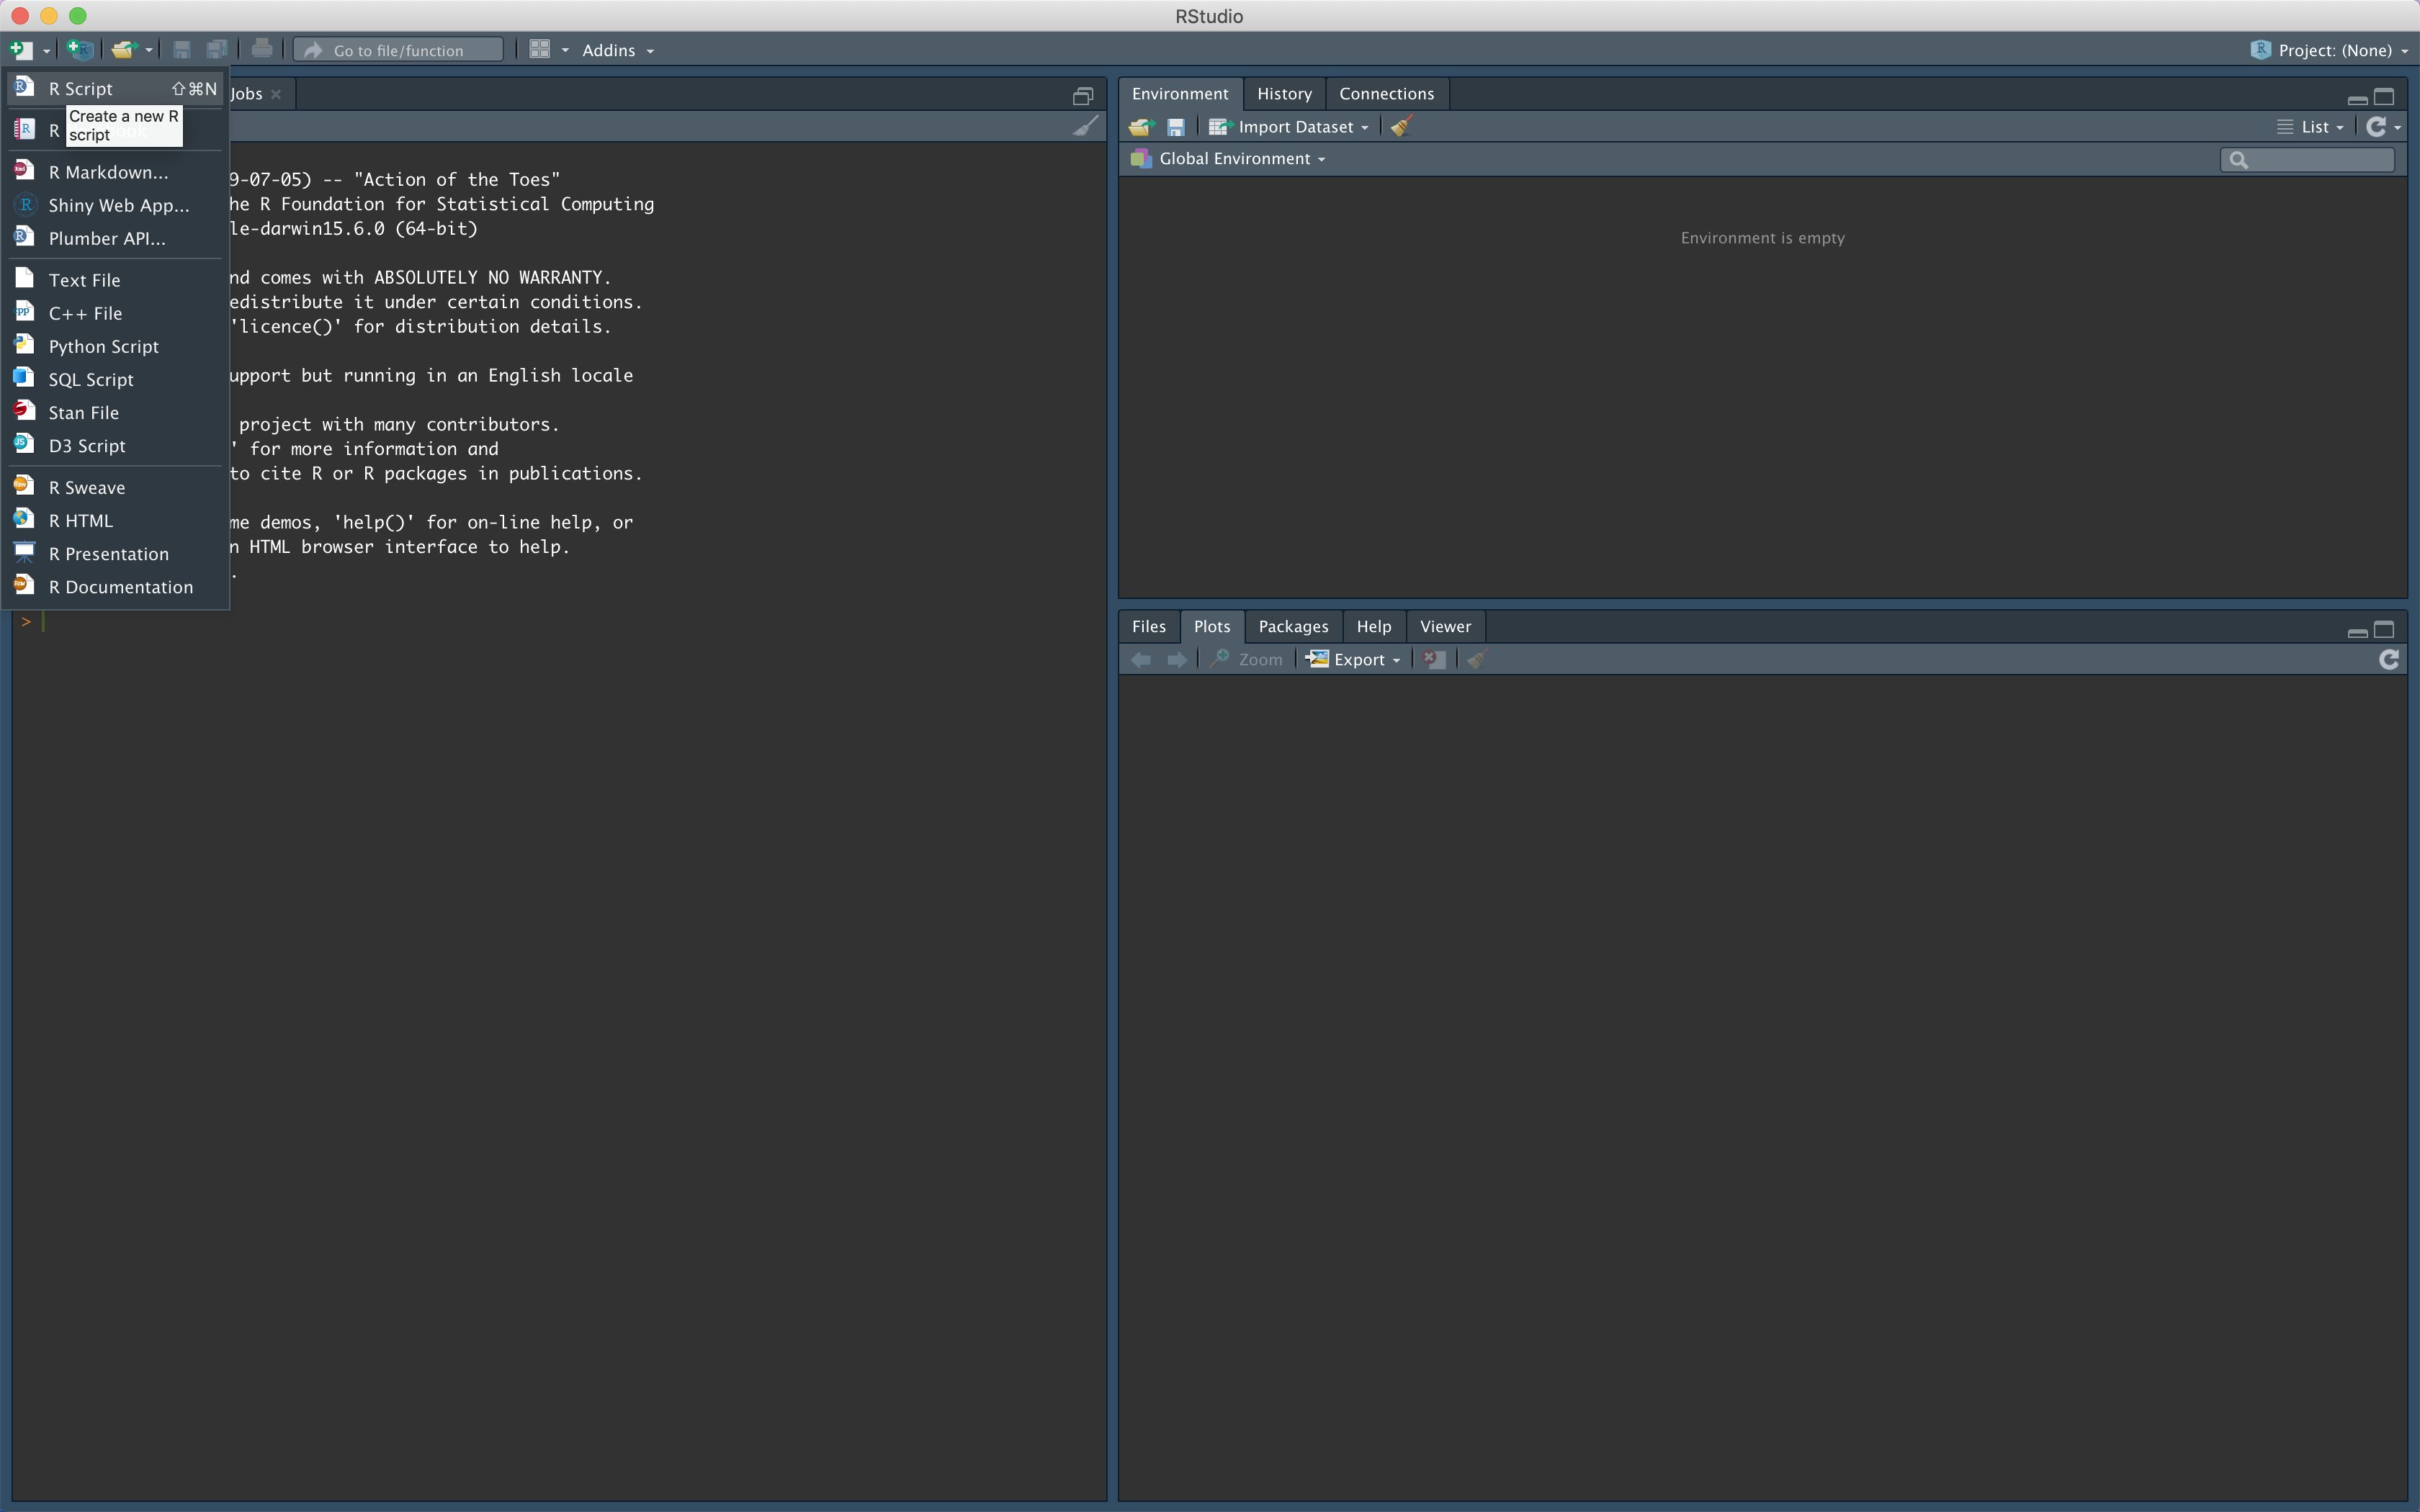
\includegraphics{Images/open_script.png}

In the script you have opened, you now need to enter a command to set
the working directory. For simplicitly, you can set your directory to
the desktop. If you are working on a Mac, you will need to type
something like the following:

\begin{Shaded}
\begin{Highlighting}[]
\FunctionTok{setwd}\NormalTok{(}\StringTok{"/Users/username/Desktop"}\NormalTok{)}
\end{Highlighting}
\end{Shaded}

If you are working on a Windows computer, you will need to type
something like the following:

\begin{Shaded}
\begin{Highlighting}[]
\FunctionTok{setwd}\NormalTok{(}\StringTok{"C:\textbackslash{}Users\textbackslash{}username\textbackslash{}Desktop"}\NormalTok{)}
\end{Highlighting}
\end{Shaded}

You will need to adapt the code I've provided above to match the naming
conventions on your machine (i.e., substitute in your own username,
etc). Google how to set your working directory if you run into any
issues. On my machine - a Mac - I type and run the following line of
code:

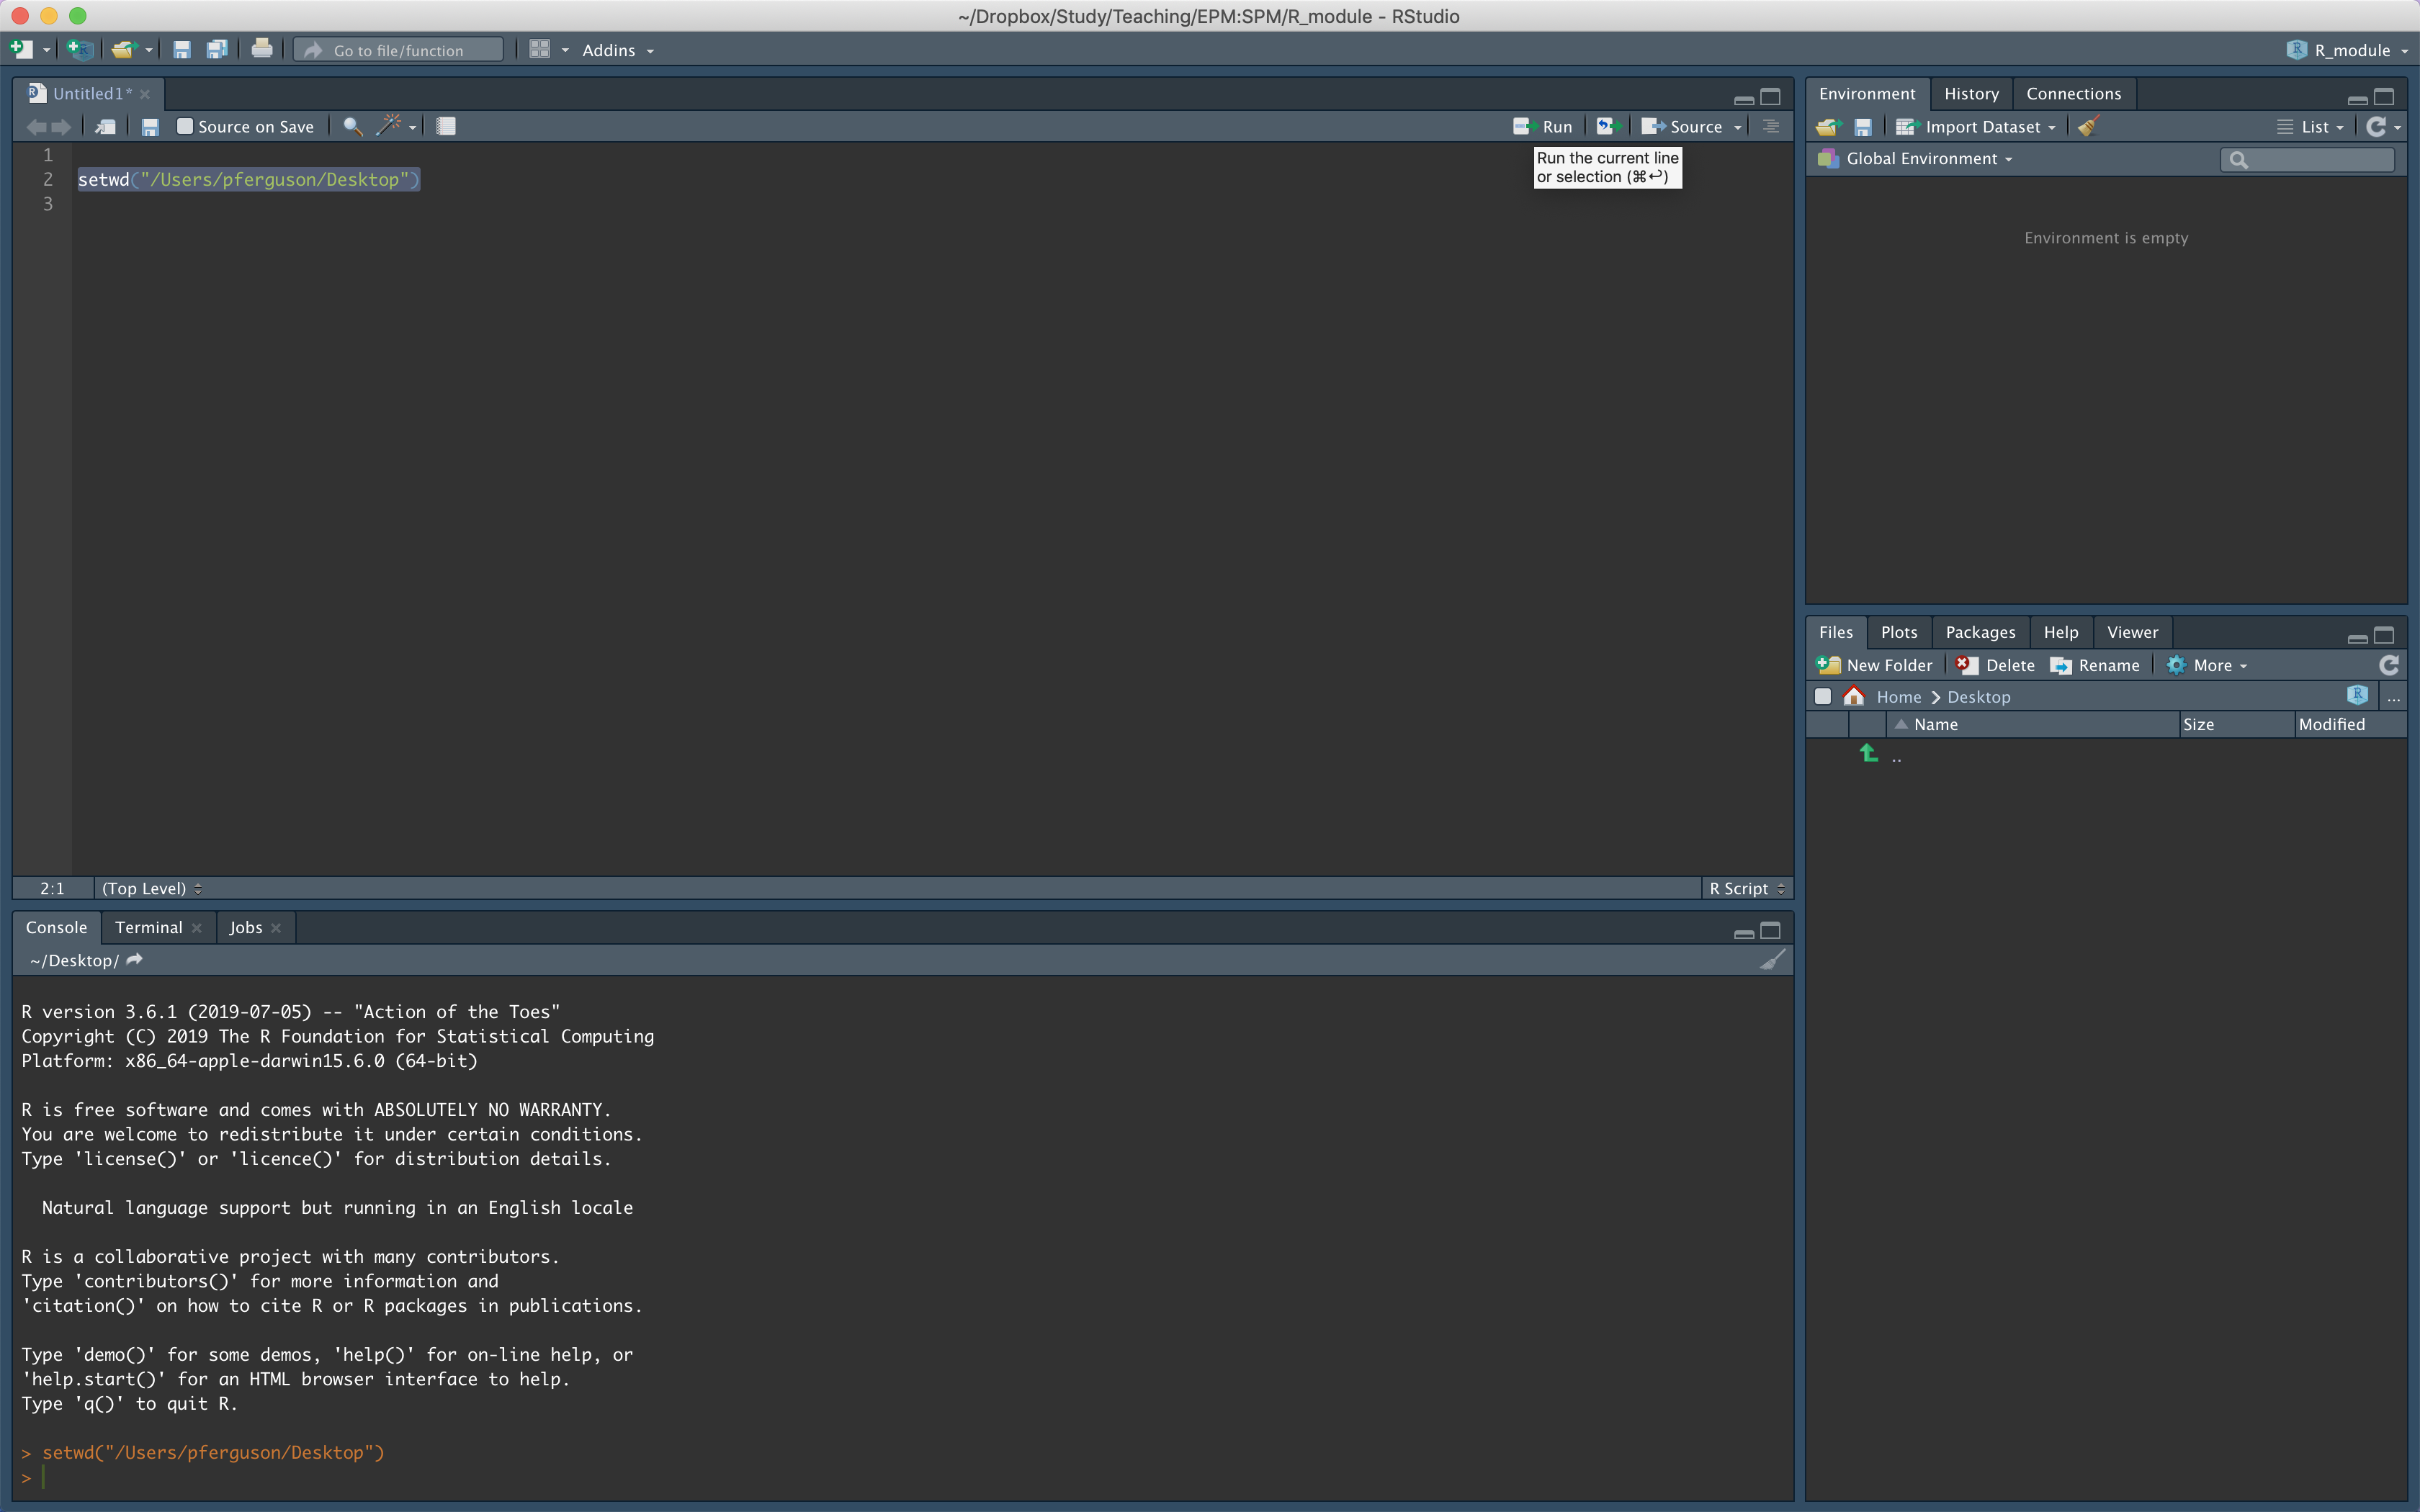
\includegraphics{Images/run_set_wd.png}

As shown in the screenshot above, to run a chunk of code in the editor,
simply select the line/s of code you want to run and then click on the
\texttt{Run} icon in the source editor pane (alternatively, if you are
on a Mac, you can highlight the code and hit \texttt{Ctrl+Enter}). You
will see the same line of code show up in the console pane below the
source editor (if it is accompanied by an error message, something has
gone wrong and your working directory will not be set to the desktop).

Having set your working directory, you now want to store the raw data
file we will be working with on the desktop.

First, you need to download the AFL data set from the course website on
the LMS. The data set can also be accessed from the \texttt{Preparation}
folder on the Github page for this module (click on
\texttt{AFL\_data\_set.csv} then click \texttt{Raw}; copy and paste the
contents to a plain text file and save as \texttt{AFL\_data\_set.csv} on
your desktop).

Next, you need to move this file to the desktop on your computer. Once
you have done this, the data set should show up as a csv file in the
browser pane of your RStudio interface.

You want to see something that looks like the following:

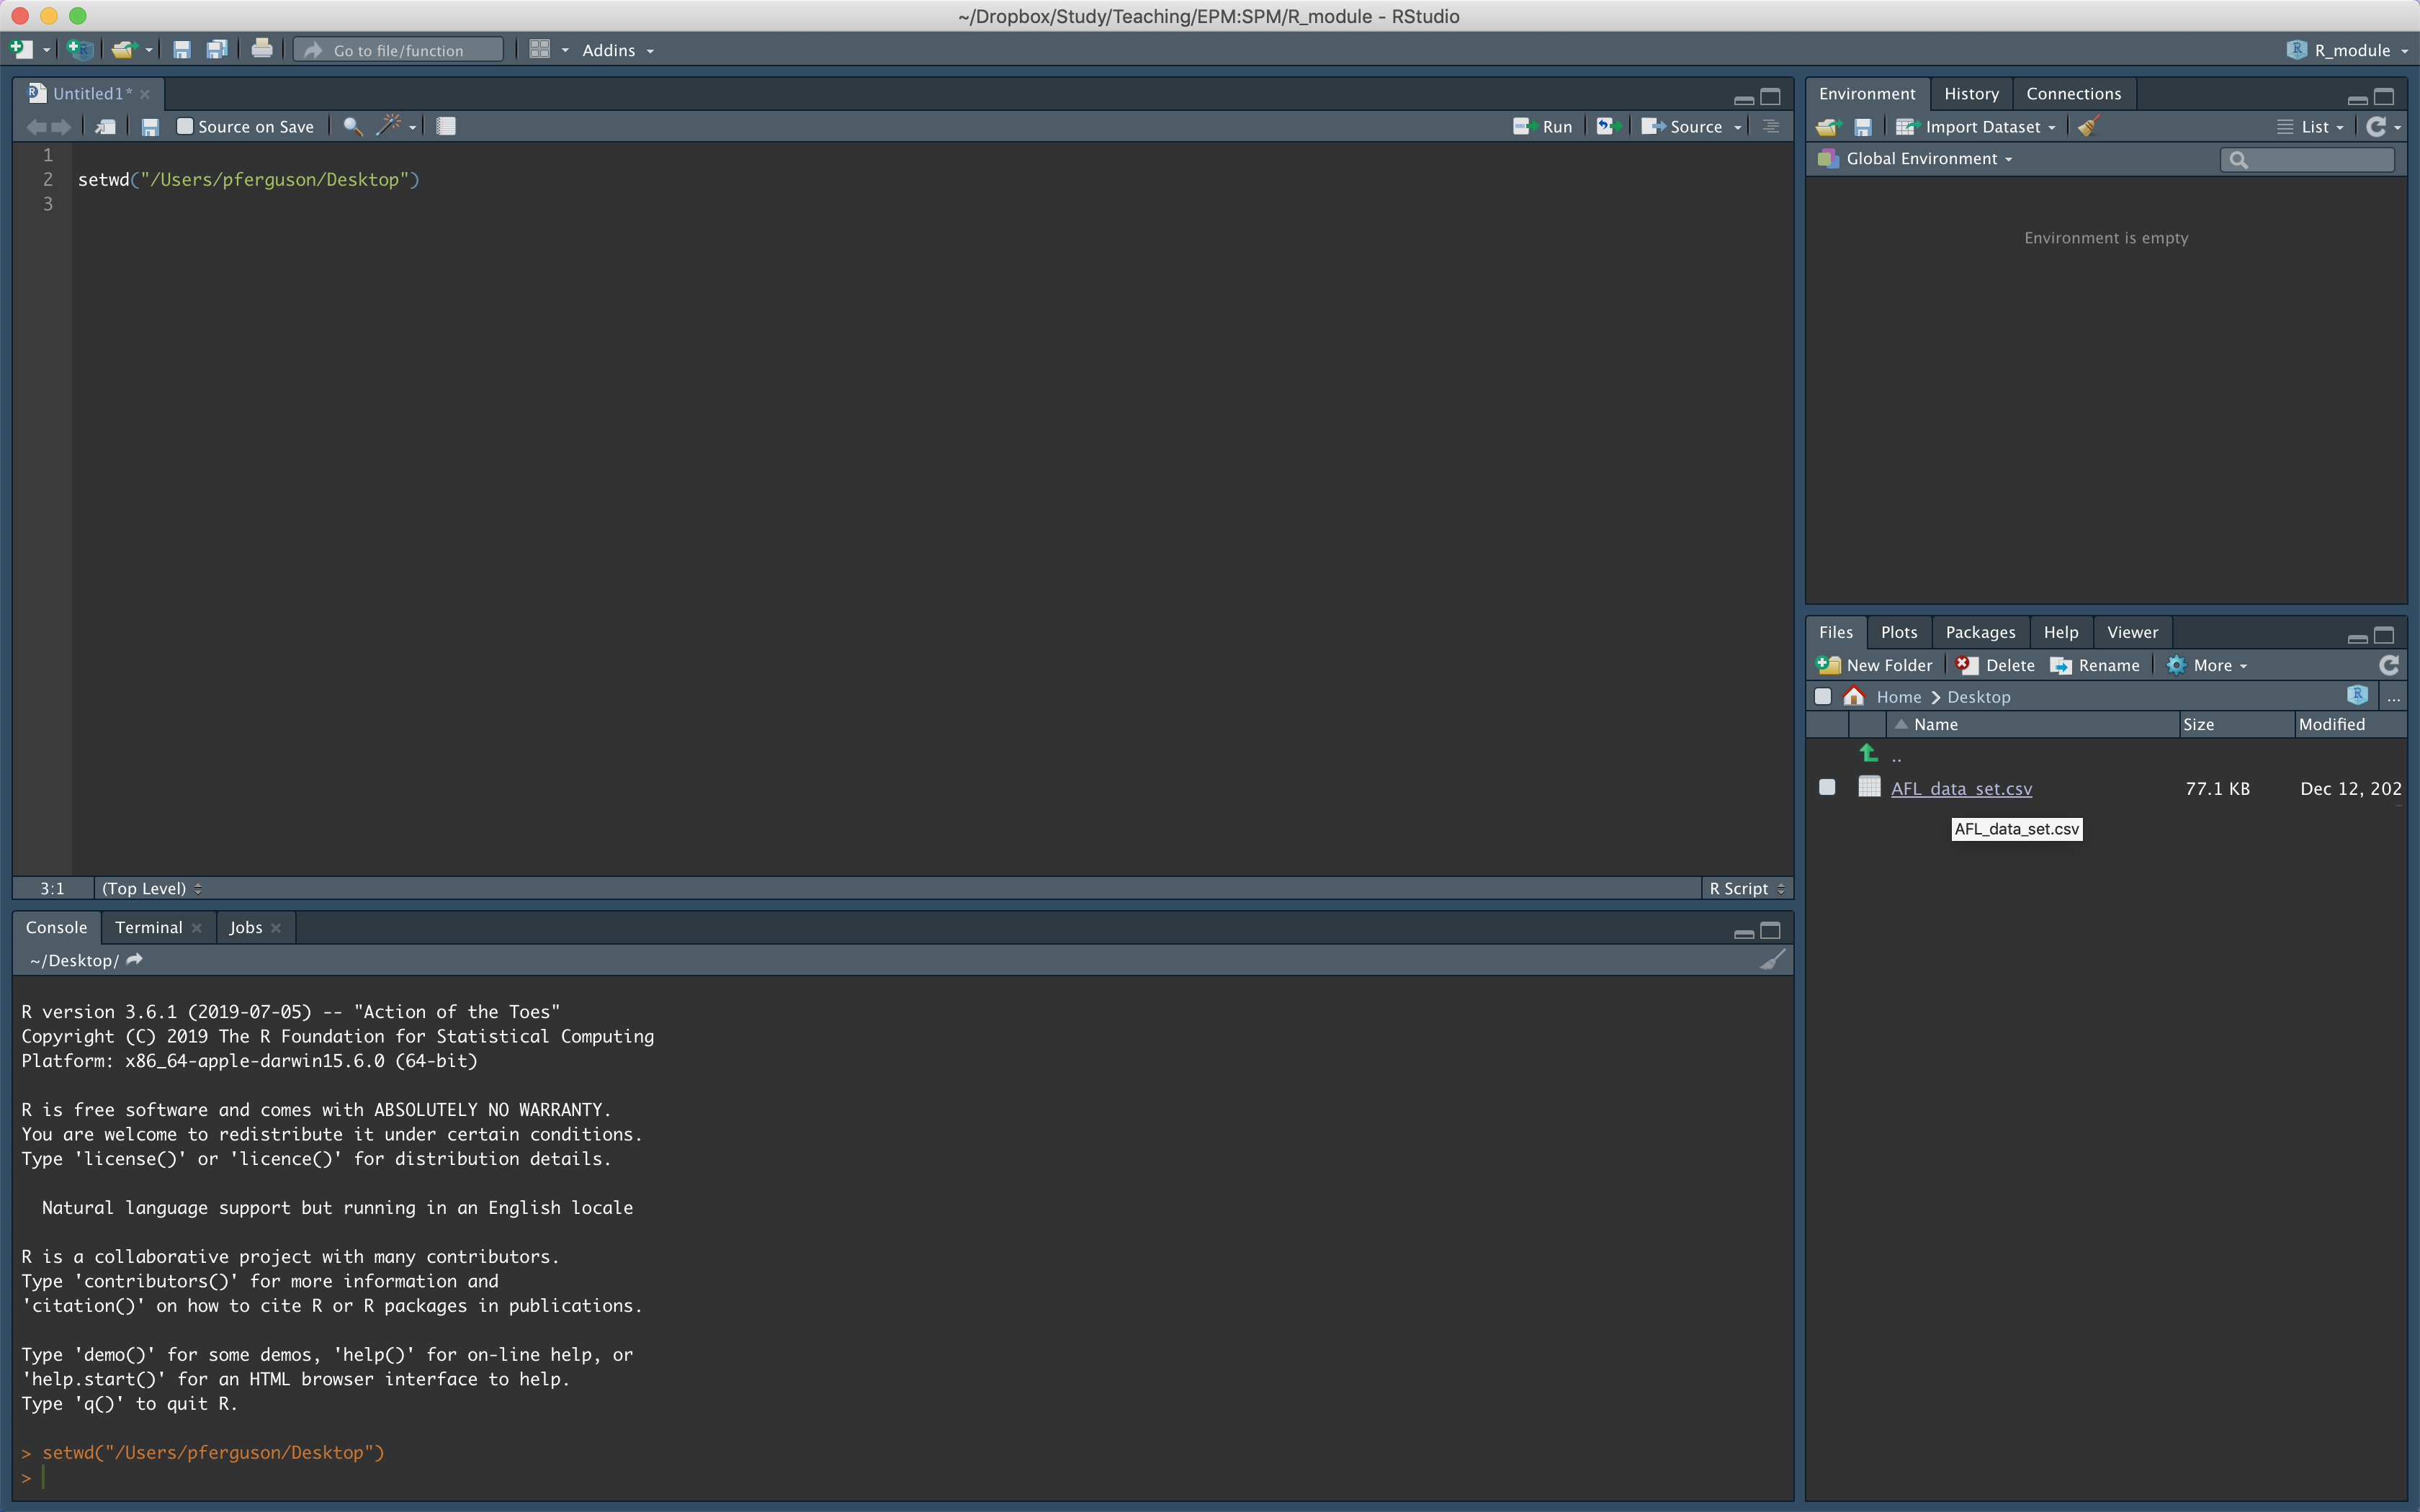
\includegraphics{Images/download_data.png}

\hypertarget{install-and-load-packages}{%
\subsubsection{Install and load
packages}\label{install-and-load-packages}}

As I mentioned in my lecture, you will primarily be working with the
`tidyverse' set of packages. As such, you will need to install and load
the tidyverse package. Installing packages in R is straight-forward and
follows the same basic convention: specify the name of the package you
want to install in the \texttt{install.packages()} function.

To install the tidyverse package, you will need to type the following
line of code in your script and hit run (just like I showed you above
when you set the working directory):

\begin{Shaded}
\begin{Highlighting}[]
\FunctionTok{install.packages}\NormalTok{(}\StringTok{"tidyverse"}\NormalTok{)}
\end{Highlighting}
\end{Shaded}

Once you have run this line of code, you should see some output show up
in the console. This output will identify the package you are
downloading and provide you with some additional information. Now that
you have installed the tidyverse package, you now need to load this
package for use. To do so, you need to run the following line of code:

\begin{Shaded}
\begin{Highlighting}[]
\FunctionTok{library}\NormalTok{(tidyverse)}
\end{Highlighting}
\end{Shaded}

Great. You are now ready to get your hands dirty. One final thing I will
mention is that you do not need to install a package every time you want
to use it. Once a packaged has been installed, it remains on your local
machine (unless you choose to remove it). However, you do need to load
installed packages each time you start a new session in R. A good habit
to get into is to start each of your scripts with a chunk of code that
loads all the packages that you commonly use.

\hypertarget{load-data-set}{%
\subsubsection{Load data set}\label{load-data-set}}

You can now load the AFL data set. To do so, copy and paste the
following line of code into your script and run it in from the source
editor:

\begin{Shaded}
\begin{Highlighting}[]
\NormalTok{AFL\_data\_set }\OtherTok{\textless{}{-}} \FunctionTok{read\_csv}\NormalTok{(}\StringTok{"AFL\_data\_set.csv"}\NormalTok{)}
\end{Highlighting}
\end{Shaded}

Most of the code you will write in R follows this same basic structure:
you are using a function - \texttt{read\_csv()} - to transform an input
(our raw data from the csv file) - into an R object - the `tibble'
(i.e., the tidy-version of a data frame), \texttt{AFL\_data\_set}.

\begin{Shaded}
\begin{Highlighting}[]
\NormalTok{AFL\_data\_set }\OtherTok{\textless{}{-}} \FunctionTok{read\_csv}\NormalTok{(}\StringTok{"AFL\_data\_set.csv"}\NormalTok{)}
\end{Highlighting}
\end{Shaded}

If all goes as planned, you should see \texttt{AFL\_data\_set} show up
in the environment pane:

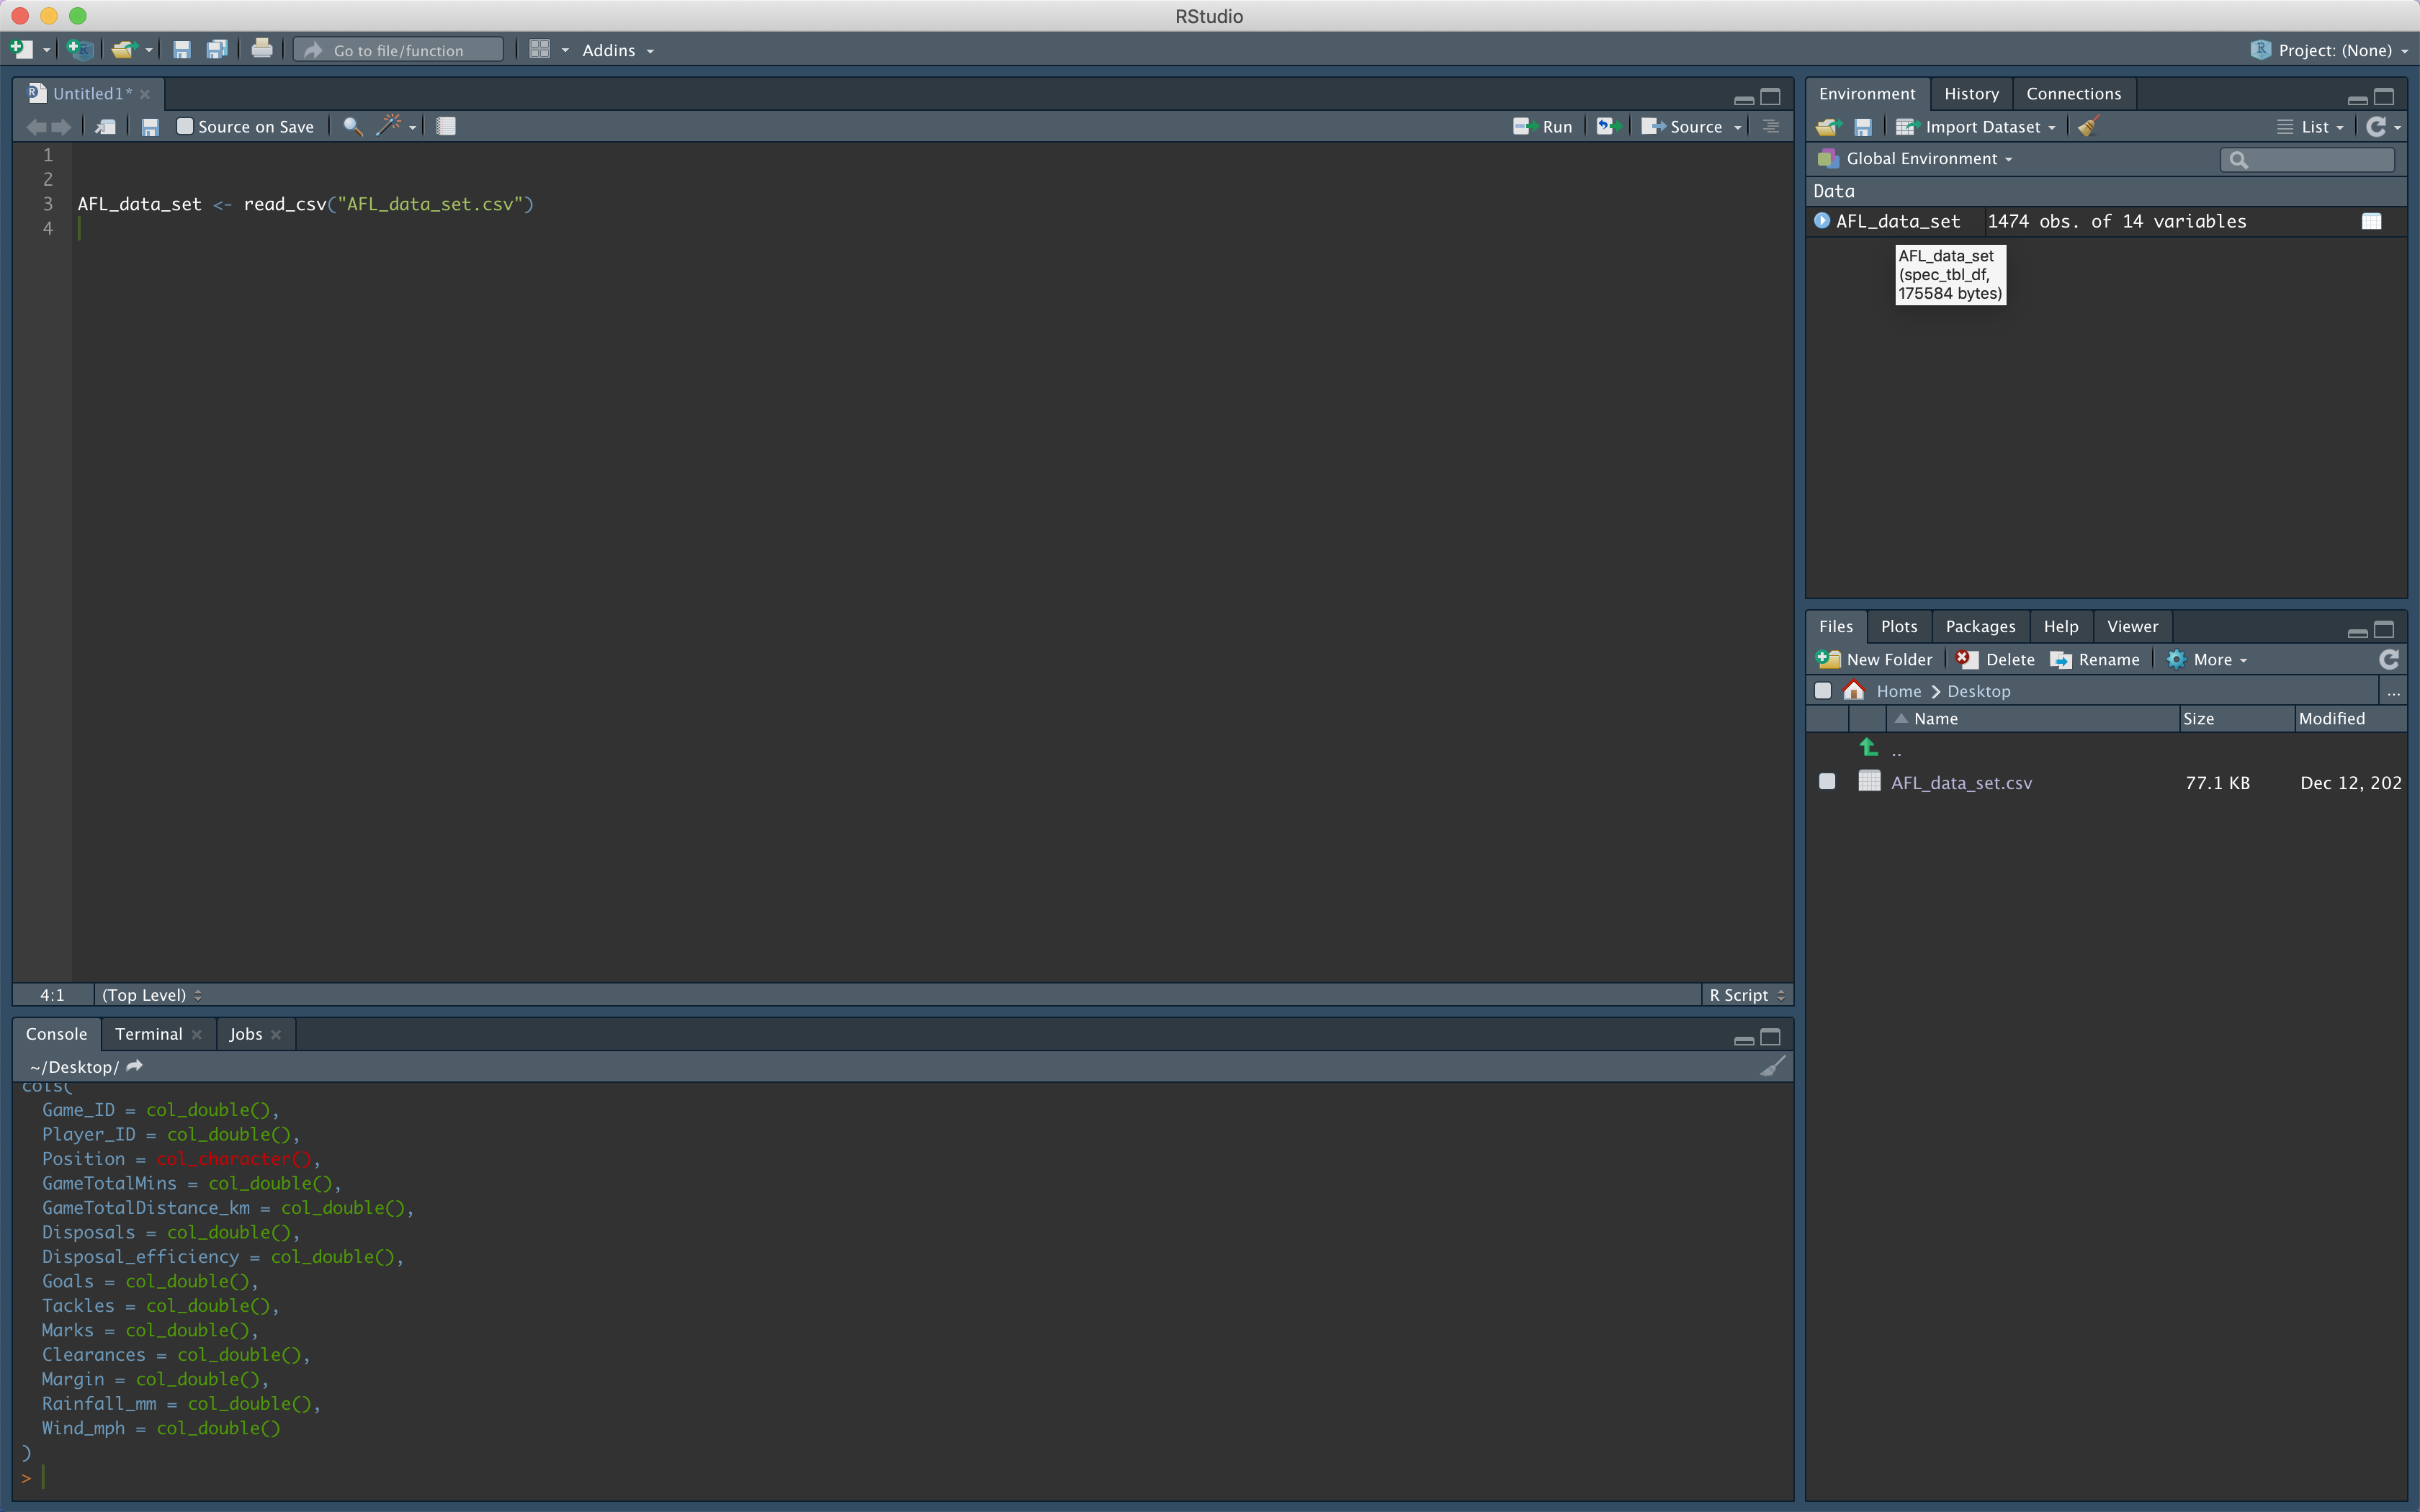
\includegraphics{Images/enviro_pane.png}

If you click on \texttt{AFL\_data\_set}, a spreadsheet-style viewer will
display the data in the source editor:

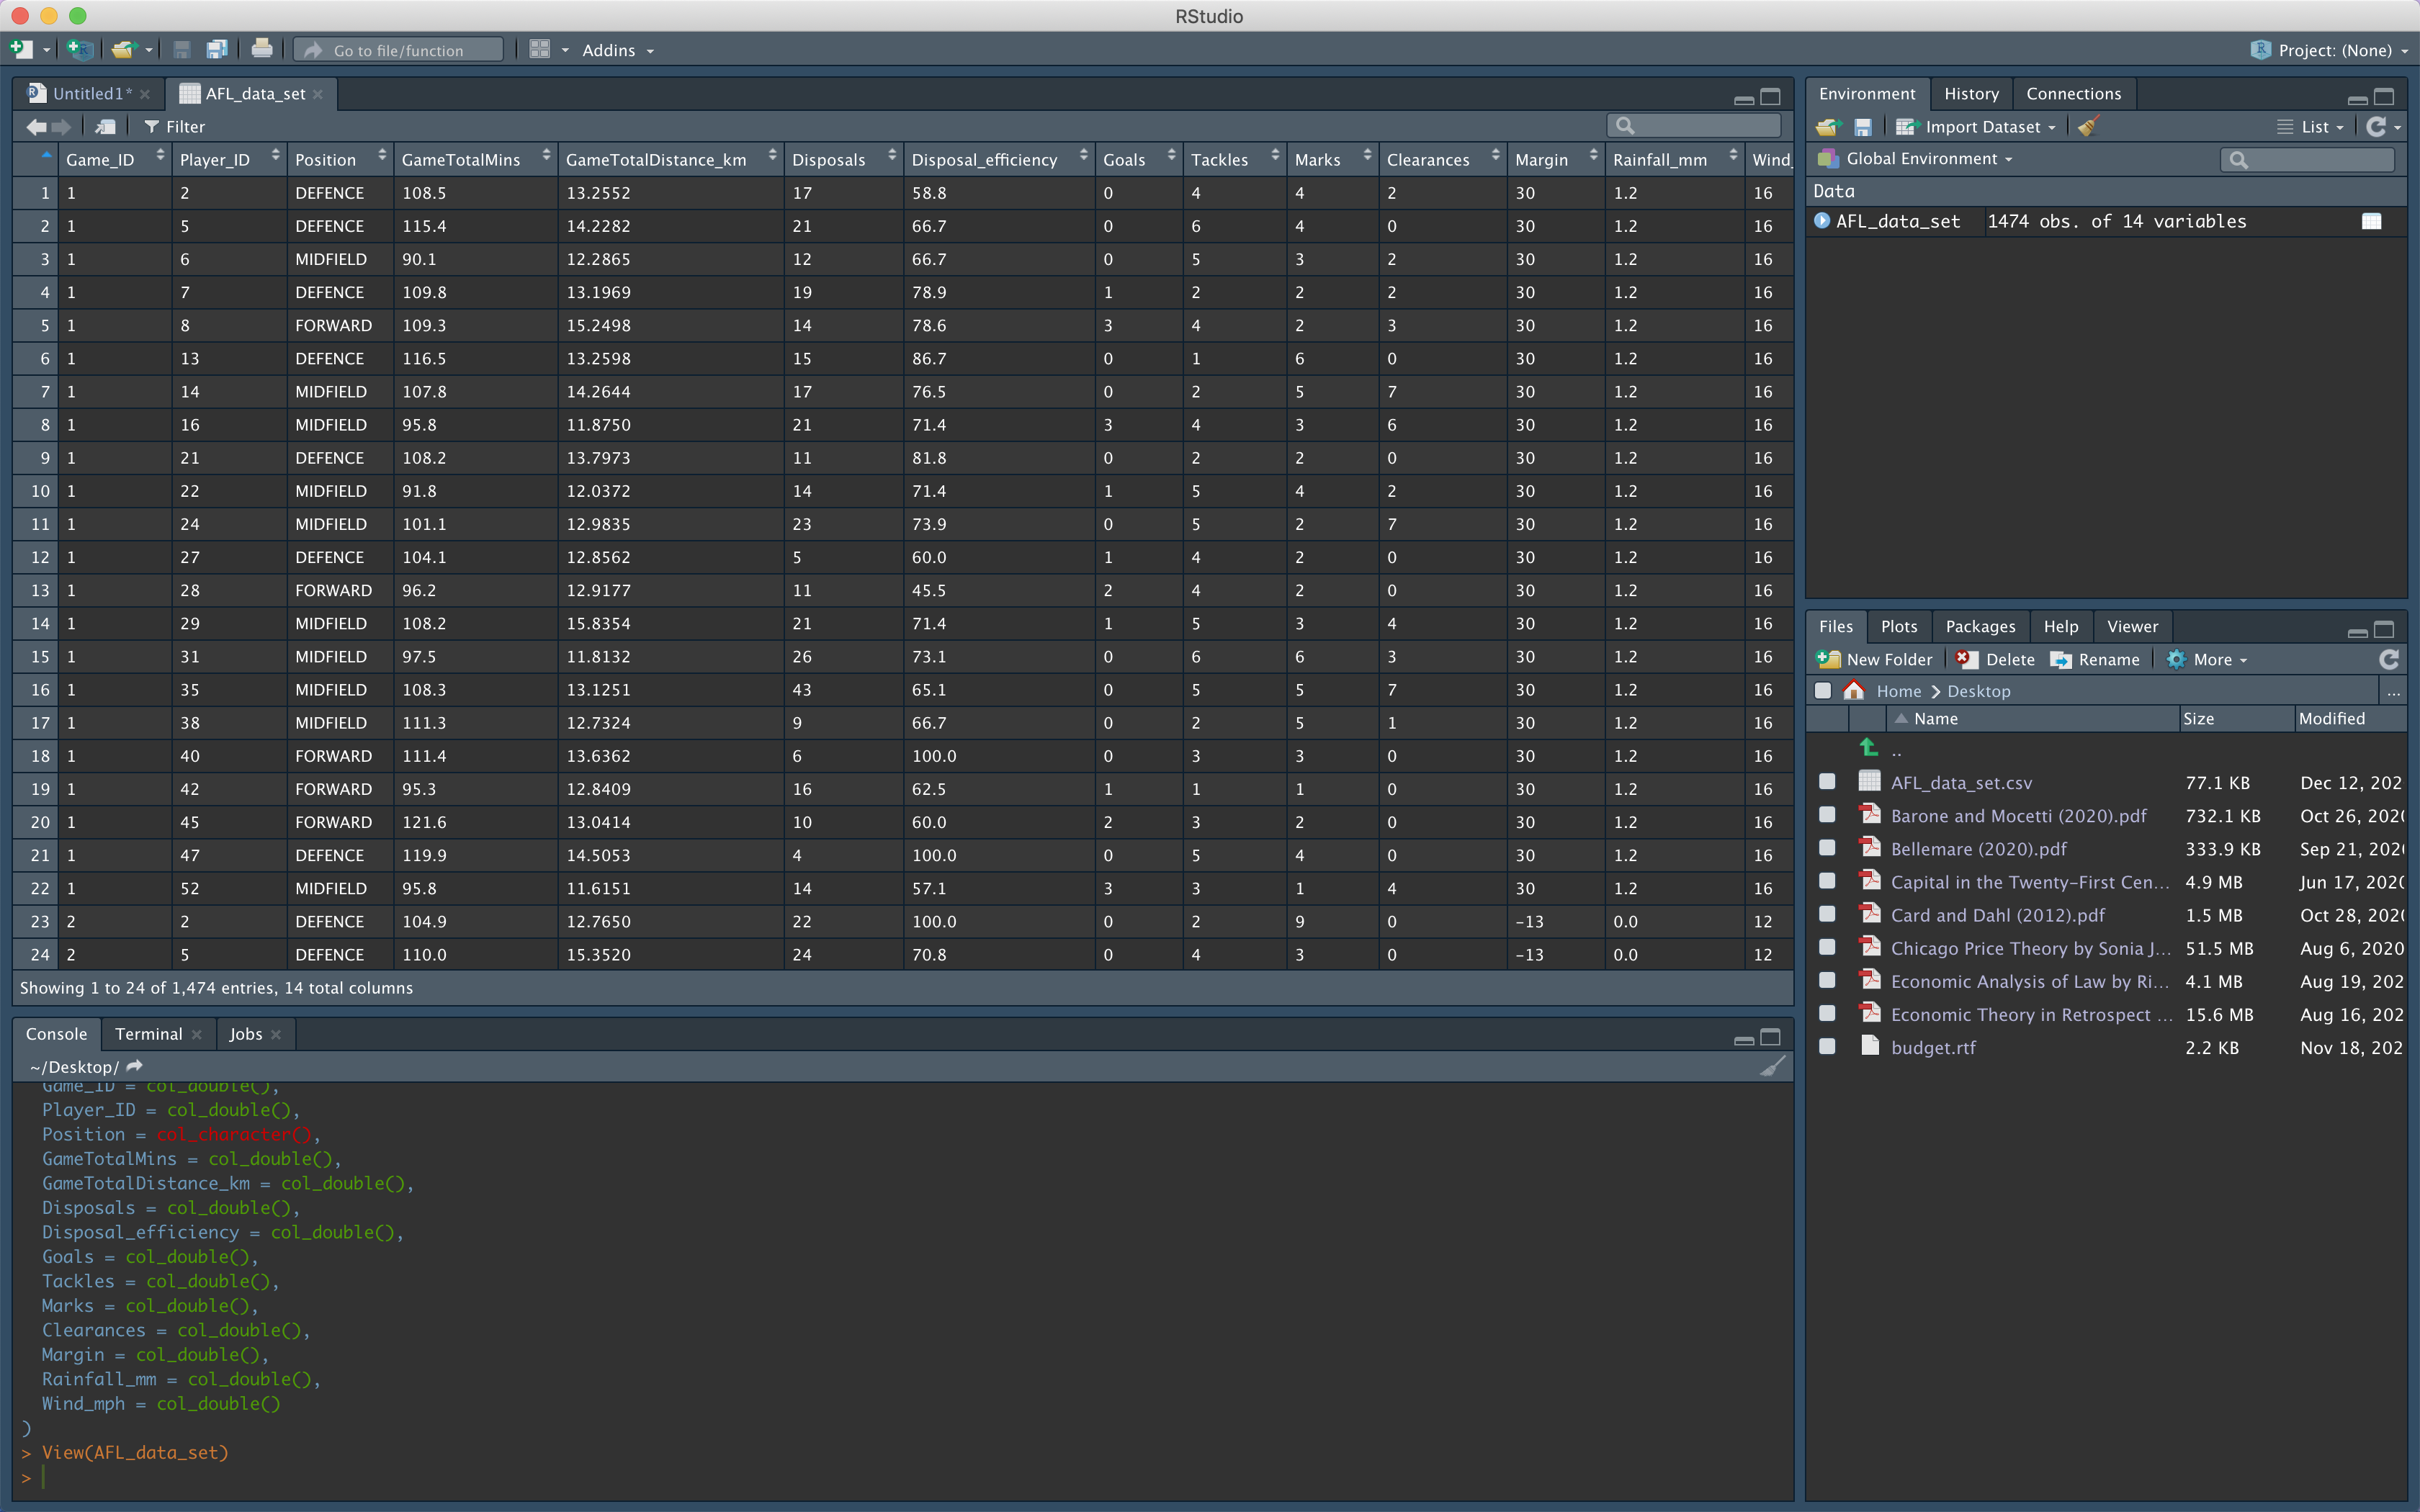
\includegraphics{Images/viewer.png}

This spreadsheet looks much like what you see when you work with data in
Excel. However, unlike with Excel, in R, we do not use point-and-click
to interact with the data. Instead, we write pieces of code. This is
appealing because code is transparent and fully replicable.

\hypertarget{examine-the-contents-and-structure-of-the-data-set}{%
\subsubsection{Examine the contents and structure of the data
set}\label{examine-the-contents-and-structure-of-the-data-set}}

Alternatively, to get a snapshot of the first ten rows of the data set,
as well as a description of its structure and contents, you can simply
type the name of the object into your script and hit run:

\begin{Shaded}
\begin{Highlighting}[]
\NormalTok{AFL\_data\_set}
\end{Highlighting}
\end{Shaded}

\begin{verbatim}
## # A tibble: 1,474 x 14
##    Game_ID Player_ID Position GameTotalMins GameTotalDistan… Disposals
##      <dbl>     <dbl> <chr>            <dbl>            <dbl>     <dbl>
##  1       1         2 DEFENCE          108.              13.3        17
##  2       1         5 DEFENCE          115.              14.2        21
##  3       1         6 MIDFIELD          90.1             12.3        12
##  4       1         7 DEFENCE          110.              13.2        19
##  5       1         8 FORWARD          109.              15.2        14
##  6       1        13 DEFENCE          116.              13.3        15
##  7       1        14 MIDFIELD         108.              14.3        17
##  8       1        16 MIDFIELD          95.8             11.9        21
##  9       1        21 DEFENCE          108.              13.8        11
## 10       1        22 MIDFIELD          91.8             12.0        14
## # … with 1,464 more rows, and 8 more variables: Disposal_efficiency <dbl>,
## #   Goals <dbl>, Tackles <dbl>, Marks <dbl>, Clearances <dbl>,
## #   Margin <dbl>, Rainfall_mm <dbl>, Wind_mph <dbl>
\end{verbatim}

You should see some output (a crude table) pop up in your console. What
can we learn from this output?

\begin{itemize}
\tightlist
\item
  The top row tells us that the object \texttt{AFL\_data\_set} is a
  tibble of dimensions 1474x14. That is, our data set contains 1474 rows
  (or observations) and 14 variables (or measures).

  \begin{itemize}
  \tightlist
  \item
    As I explained in class, each row is a player-game observation
    (i.e., a player's performance measures for an individual game).
  \end{itemize}
\item
  The second row down gives us the names of the first six variables in
  our data set. The notes at the bottom of the table tell us that there
  are `8 more variables' not reported in the output.

  \begin{itemize}
  \tightlist
  \item
    This is a limit of viewing a data set in this fashion: if the data
    set is `too wide', you only see the first few variables.
  \end{itemize}
\item
  The third row down tells us the `types' of variables in our data set.
  You can think of \texttt{dbl} as a number, and you can think of
  \texttt{chr} as words.
\item
  From the fourth row down, you can see the actual data (or
  observations) in our data set.
\end{itemize}

While this output provides a useful overview of our data set, another
helpful way to explore our data is to run the following command, which
outputs the first ten rows of the data in a slightly easier-to-read
structure:

\begin{Shaded}
\begin{Highlighting}[]
\NormalTok{knitr}\SpecialCharTok{::}\FunctionTok{kable}\NormalTok{(AFL\_data\_set[}\DecValTok{1}\SpecialCharTok{:}\DecValTok{10}\NormalTok{,])}
\end{Highlighting}
\end{Shaded}

\begin{longtable}[]{@{}
  >{\raggedleft\arraybackslash}p{(\columnwidth - 26\tabcolsep) * \real{0.06}}
  >{\raggedleft\arraybackslash}p{(\columnwidth - 26\tabcolsep) * \real{0.07}}
  >{\raggedright\arraybackslash}p{(\columnwidth - 26\tabcolsep) * \real{0.06}}
  >{\raggedleft\arraybackslash}p{(\columnwidth - 26\tabcolsep) * \real{0.09}}
  >{\raggedleft\arraybackslash}p{(\columnwidth - 26\tabcolsep) * \real{0.15}}
  >{\raggedleft\arraybackslash}p{(\columnwidth - 26\tabcolsep) * \real{0.06}}
  >{\raggedleft\arraybackslash}p{(\columnwidth - 26\tabcolsep) * \real{0.14}}
  >{\raggedleft\arraybackslash}p{(\columnwidth - 26\tabcolsep) * \real{0.03}}
  >{\raggedleft\arraybackslash}p{(\columnwidth - 26\tabcolsep) * \real{0.05}}
  >{\raggedleft\arraybackslash}p{(\columnwidth - 26\tabcolsep) * \real{0.03}}
  >{\raggedleft\arraybackslash}p{(\columnwidth - 26\tabcolsep) * \real{0.07}}
  >{\raggedleft\arraybackslash}p{(\columnwidth - 26\tabcolsep) * \real{0.04}}
  >{\raggedleft\arraybackslash}p{(\columnwidth - 26\tabcolsep) * \real{0.08}}
  >{\raggedleft\arraybackslash}p{(\columnwidth - 26\tabcolsep) * \real{0.06}}@{}}
\toprule
Game\_ID & Player\_ID & Position & GameTotalMins & GameTotalDistance\_km
& Disposals & Disposal\_efficiency & Goals & Tackles & Marks &
Clearances & Margin & Rainfall\_mm & Wind\_mph \\
\midrule
\endhead
1 & 2 & DEFENCE & 108.5 & 13.2552 & 17 & 58.8 & 0 & 4 & 4 & 2 & 30 & 1.2
& 16 \\
1 & 5 & DEFENCE & 115.4 & 14.2282 & 21 & 66.7 & 0 & 6 & 4 & 0 & 30 & 1.2
& 16 \\
1 & 6 & MIDFIELD & 90.1 & 12.2865 & 12 & 66.7 & 0 & 5 & 3 & 2 & 30 & 1.2
& 16 \\
1 & 7 & DEFENCE & 109.8 & 13.1969 & 19 & 78.9 & 1 & 2 & 2 & 2 & 30 & 1.2
& 16 \\
1 & 8 & FORWARD & 109.3 & 15.2498 & 14 & 78.6 & 3 & 4 & 2 & 3 & 30 & 1.2
& 16 \\
1 & 13 & DEFENCE & 116.5 & 13.2598 & 15 & 86.7 & 0 & 1 & 6 & 0 & 30 &
1.2 & 16 \\
1 & 14 & MIDFIELD & 107.8 & 14.2644 & 17 & 76.5 & 0 & 2 & 5 & 7 & 30 &
1.2 & 16 \\
1 & 16 & MIDFIELD & 95.8 & 11.8750 & 21 & 71.4 & 3 & 4 & 3 & 6 & 30 &
1.2 & 16 \\
1 & 21 & DEFENCE & 108.2 & 13.7973 & 11 & 81.8 & 0 & 2 & 2 & 0 & 30 &
1.2 & 16 \\
1 & 22 & MIDFIELD & 91.8 & 12.0372 & 14 & 71.4 & 1 & 5 & 4 & 2 & 30 &
1.2 & 16 \\
\bottomrule
\end{longtable}

To get a better sense of how to interpret the contents of our data set,
I will interpret the first row reported above.

\begin{itemize}
\tightlist
\item
  In Game\_ID=1, Player\_ID=2, a defender, played 108.5 minutes of game
  time during which he ran 13.3 km. He accumulated a total of 17
  disposals, at an efficiency rate of 58.8\%. He kicked 0 goals,
  completed 4 tackles, took 5 marks, and completed 2 clearances. His
  team lost the game by 30 points. During the game, there was 1.2mm of
  rainfall, and the average windspeed was 16 miles per hour.
\end{itemize}

\hypertarget{creating-variables}{%
\subsubsection{Creating variables}\label{creating-variables}}

Now that you have a handle on our data set, I am going to get you to
create some new variables. You will use the function \texttt{mutate()}
to create these variables. I will also get you to use pipes
(\%\textgreater\%) to string together pieces of code. You should get in
the habit of using pipes. They can help you to compartmentalize blocks
of complex code. Pipes also make your code easier to read - something
you will appreciate if you ever have to return to and work with a piece
of code you wrote in the distant past.

First, I will get you to create a variable that measures running
distance in meters per minute of game time. To generate this variable,
you need to run the following chunk of code:

\begin{Shaded}
\begin{Highlighting}[]
\NormalTok{AFL\_data\_set }\OtherTok{\textless{}{-}}\NormalTok{ AFL\_data\_set }\SpecialCharTok{\%\textgreater{}\%}
  \FunctionTok{mutate}\NormalTok{(}\AttributeTok{Meters\_per\_min=}\NormalTok{(GameTotalDistance\_km}\SpecialCharTok{*}\DecValTok{1000}\NormalTok{)}\SpecialCharTok{/}\NormalTok{GameTotalMins)}
\end{Highlighting}
\end{Shaded}

Second, I will get you to create a variable that indicates (i.e., takes
a value of one) if a player kicked 2+ goals in a game and also ran 14+
km. To generate this variable - which we will call
\texttt{best\_on\_ground} - you need to run the following chunk of code:

\begin{Shaded}
\begin{Highlighting}[]
\NormalTok{AFL\_data\_set }\OtherTok{\textless{}{-}}\NormalTok{ AFL\_data\_set }\SpecialCharTok{\%\textgreater{}\%}
  \FunctionTok{mutate}\NormalTok{(}\AttributeTok{best\_on\_ground=}\FunctionTok{ifelse}\NormalTok{(Goals }\SpecialCharTok{\textgreater{}=} \DecValTok{2} \SpecialCharTok{\&}\NormalTok{ GameTotalDistance\_km }\SpecialCharTok{\textgreater{}=} \DecValTok{14}\NormalTok{, }\DecValTok{1}\NormalTok{, }\DecValTok{0}\NormalTok{))}
\end{Highlighting}
\end{Shaded}

To confirm that your code ran as intended, you should take another quick
look at your data set to confirm that the new variables now show up:

\begin{Shaded}
\begin{Highlighting}[]
\NormalTok{knitr}\SpecialCharTok{::}\FunctionTok{kable}\NormalTok{(AFL\_data\_set[}\DecValTok{1}\SpecialCharTok{:}\DecValTok{10}\NormalTok{,])}
\end{Highlighting}
\end{Shaded}

\begin{longtable}[]{@{}
  >{\raggedleft\arraybackslash}p{(\columnwidth - 30\tabcolsep) * \real{0.05}}
  >{\raggedleft\arraybackslash}p{(\columnwidth - 30\tabcolsep) * \real{0.06}}
  >{\raggedright\arraybackslash}p{(\columnwidth - 30\tabcolsep) * \real{0.05}}
  >{\raggedleft\arraybackslash}p{(\columnwidth - 30\tabcolsep) * \real{0.07}}
  >{\raggedleft\arraybackslash}p{(\columnwidth - 30\tabcolsep) * \real{0.12}}
  >{\raggedleft\arraybackslash}p{(\columnwidth - 30\tabcolsep) * \real{0.05}}
  >{\raggedleft\arraybackslash}p{(\columnwidth - 30\tabcolsep) * \real{0.11}}
  >{\raggedleft\arraybackslash}p{(\columnwidth - 30\tabcolsep) * \real{0.03}}
  >{\raggedleft\arraybackslash}p{(\columnwidth - 30\tabcolsep) * \real{0.04}}
  >{\raggedleft\arraybackslash}p{(\columnwidth - 30\tabcolsep) * \real{0.03}}
  >{\raggedleft\arraybackslash}p{(\columnwidth - 30\tabcolsep) * \real{0.06}}
  >{\raggedleft\arraybackslash}p{(\columnwidth - 30\tabcolsep) * \real{0.03}}
  >{\raggedleft\arraybackslash}p{(\columnwidth - 30\tabcolsep) * \real{0.07}}
  >{\raggedleft\arraybackslash}p{(\columnwidth - 30\tabcolsep) * \real{0.05}}
  >{\raggedleft\arraybackslash}p{(\columnwidth - 30\tabcolsep) * \real{0.09}}
  >{\raggedleft\arraybackslash}p{(\columnwidth - 30\tabcolsep) * \real{0.09}}@{}}
\toprule
Game\_ID & Player\_ID & Position & GameTotalMins & GameTotalDistance\_km
& Disposals & Disposal\_efficiency & Goals & Tackles & Marks &
Clearances & Margin & Rainfall\_mm & Wind\_mph & Meters\_per\_min &
best\_on\_ground \\
\midrule
\endhead
1 & 2 & DEFENCE & 108.5 & 13.2552 & 17 & 58.8 & 0 & 4 & 4 & 2 & 30 & 1.2
& 16 & 122.1677 & 0 \\
1 & 5 & DEFENCE & 115.4 & 14.2282 & 21 & 66.7 & 0 & 6 & 4 & 0 & 30 & 1.2
& 16 & 123.2946 & 0 \\
1 & 6 & MIDFIELD & 90.1 & 12.2865 & 12 & 66.7 & 0 & 5 & 3 & 2 & 30 & 1.2
& 16 & 136.3651 & 0 \\
1 & 7 & DEFENCE & 109.8 & 13.1969 & 19 & 78.9 & 1 & 2 & 2 & 2 & 30 & 1.2
& 16 & 120.1903 & 0 \\
1 & 8 & FORWARD & 109.3 & 15.2498 & 14 & 78.6 & 3 & 4 & 2 & 3 & 30 & 1.2
& 16 & 139.5224 & 1 \\
1 & 13 & DEFENCE & 116.5 & 13.2598 & 15 & 86.7 & 0 & 1 & 6 & 0 & 30 &
1.2 & 16 & 113.8180 & 0 \\
1 & 14 & MIDFIELD & 107.8 & 14.2644 & 17 & 76.5 & 0 & 2 & 5 & 7 & 30 &
1.2 & 16 & 132.3228 & 0 \\
1 & 16 & MIDFIELD & 95.8 & 11.8750 & 21 & 71.4 & 3 & 4 & 3 & 6 & 30 &
1.2 & 16 & 123.9562 & 0 \\
1 & 21 & DEFENCE & 108.2 & 13.7973 & 11 & 81.8 & 0 & 2 & 2 & 0 & 30 &
1.2 & 16 & 127.5166 & 0 \\
1 & 22 & MIDFIELD & 91.8 & 12.0372 & 14 & 71.4 & 1 & 5 & 4 & 2 & 30 &
1.2 & 16 & 131.1242 & 0 \\
\bottomrule
\end{longtable}

You should seem them as the final two columns in the data set.

\hypertarget{subsetting-our-data}{%
\subsubsection{Subsetting our data}\label{subsetting-our-data}}

When you have large data sets, you will often only want to look at a
subset or snapshot of your data. In the case of wide data sets (i.e.,
many columns), you may want to only look at or work with a subset of
variables. In the case of long data sets (i.e., many rows), you may want
to only look at or work with a subset of observations.

You can use the function \texttt{select()} to `narrow' a wide data set
(i.e., drop variables). For example, let's say we want to create a
tibble that contains the following four variables from our AFL data set:
\texttt{Player\_ID}, \texttt{Game\_ID}, and the two new variables we
just created - \texttt{Meters\_per\_min} and \texttt{best\_on\_ground}.
You can run the following code to create this `narrow' data set:

\begin{Shaded}
\begin{Highlighting}[]
\NormalTok{narrow }\OtherTok{\textless{}{-}}\NormalTok{ AFL\_data\_set }\SpecialCharTok{\%\textgreater{}\%}
  \FunctionTok{select}\NormalTok{(Player\_ID, Game\_ID, Meters\_per\_min, best\_on\_ground)}
\end{Highlighting}
\end{Shaded}

If we take a quick peek at this new tibble, you can see that it contains
only the four variables that we wanted from our original, wider data
set:

\begin{Shaded}
\begin{Highlighting}[]
\NormalTok{knitr}\SpecialCharTok{::}\FunctionTok{kable}\NormalTok{(narrow[}\DecValTok{1}\SpecialCharTok{:}\DecValTok{10}\NormalTok{,])}
\end{Highlighting}
\end{Shaded}

\begin{longtable}[]{@{}rrrr@{}}
\toprule
Player\_ID & Game\_ID & Meters\_per\_min & best\_on\_ground \\
\midrule
\endhead
2 & 1 & 122.1677 & 0 \\
5 & 1 & 123.2946 & 0 \\
6 & 1 & 136.3651 & 0 \\
7 & 1 & 120.1903 & 0 \\
8 & 1 & 139.5224 & 1 \\
13 & 1 & 113.8180 & 0 \\
14 & 1 & 132.3228 & 0 \\
16 & 1 & 123.9562 & 0 \\
21 & 1 & 127.5166 & 0 \\
22 & 1 & 131.1242 & 0 \\
\bottomrule
\end{longtable}

If you want to `shorten' a long data set (i.e, drop observations), you
can use the \texttt{filter()} command. For example, the following piece
of code creates a tibble that only contains observations from our AFL
data set for which \texttt{best\_on\_ground=1} (i.e., observations where
the player scored 2+ goals in the game and ran more than 14 km):

\begin{Shaded}
\begin{Highlighting}[]
\NormalTok{short }\OtherTok{\textless{}{-}}\NormalTok{ AFL\_data\_set }\SpecialCharTok{\%\textgreater{}\%}
  \FunctionTok{filter}\NormalTok{(best\_on\_ground}\SpecialCharTok{==}\DecValTok{1}\NormalTok{)}
\end{Highlighting}
\end{Shaded}

You should then be able to see that this new tibble only contains
observations from the AFL data set for which
\texttt{best\_on\_ground=1}:

\begin{Shaded}
\begin{Highlighting}[]
\NormalTok{knitr}\SpecialCharTok{::}\FunctionTok{kable}\NormalTok{(short[}\DecValTok{1}\SpecialCharTok{:}\DecValTok{10}\NormalTok{,])}
\end{Highlighting}
\end{Shaded}

\begin{longtable}[]{@{}
  >{\raggedleft\arraybackslash}p{(\columnwidth - 30\tabcolsep) * \real{0.05}}
  >{\raggedleft\arraybackslash}p{(\columnwidth - 30\tabcolsep) * \real{0.06}}
  >{\raggedright\arraybackslash}p{(\columnwidth - 30\tabcolsep) * \real{0.05}}
  >{\raggedleft\arraybackslash}p{(\columnwidth - 30\tabcolsep) * \real{0.07}}
  >{\raggedleft\arraybackslash}p{(\columnwidth - 30\tabcolsep) * \real{0.12}}
  >{\raggedleft\arraybackslash}p{(\columnwidth - 30\tabcolsep) * \real{0.05}}
  >{\raggedleft\arraybackslash}p{(\columnwidth - 30\tabcolsep) * \real{0.11}}
  >{\raggedleft\arraybackslash}p{(\columnwidth - 30\tabcolsep) * \real{0.03}}
  >{\raggedleft\arraybackslash}p{(\columnwidth - 30\tabcolsep) * \real{0.04}}
  >{\raggedleft\arraybackslash}p{(\columnwidth - 30\tabcolsep) * \real{0.03}}
  >{\raggedleft\arraybackslash}p{(\columnwidth - 30\tabcolsep) * \real{0.06}}
  >{\raggedleft\arraybackslash}p{(\columnwidth - 30\tabcolsep) * \real{0.03}}
  >{\raggedleft\arraybackslash}p{(\columnwidth - 30\tabcolsep) * \real{0.07}}
  >{\raggedleft\arraybackslash}p{(\columnwidth - 30\tabcolsep) * \real{0.05}}
  >{\raggedleft\arraybackslash}p{(\columnwidth - 30\tabcolsep) * \real{0.09}}
  >{\raggedleft\arraybackslash}p{(\columnwidth - 30\tabcolsep) * \real{0.09}}@{}}
\toprule
Game\_ID & Player\_ID & Position & GameTotalMins & GameTotalDistance\_km
& Disposals & Disposal\_efficiency & Goals & Tackles & Marks &
Clearances & Margin & Rainfall\_mm & Wind\_mph & Meters\_per\_min &
best\_on\_ground \\
\midrule
\endhead
1 & 8 & FORWARD & 109.3 & 15.2498 & 14 & 78.6 & 3 & 4 & 2 & 3 & 30 & 1.2
& 16 & 139.5224 & 1 \\
2 & 29 & MIDFIELD & 99.4 & 14.4787 & 17 & 82.4 & 2 & 7 & 3 & 3 & -13 &
0.0 & 12 & 145.6610 & 1 \\
3 & 28 & FORWARD & 101.6 & 14.2604 & 13 & 92.3 & 2 & 4 & 3 & 1 & 69 &
0.0 & 9 & 140.3583 & 1 \\
3 & 42 & MIDFIELD & 104.2 & 14.3412 & 28 & 71.4 & 2 & 2 & 5 & 5 & 69 &
0.0 & 9 & 137.6315 & 1 \\
5 & 9 & FORWARD & 108.1 & 14.8046 & 18 & 72.2 & 3 & 4 & 3 & 1 & 48 & 0.0
& 4 & 136.9528 & 1 \\
5 & 28 & FORWARD & 102.2 & 14.6557 & 14 & 64.3 & 2 & 2 & 4 & 2 & 48 &
0.0 & 4 & 143.4022 & 1 \\
7 & 40 & FORWARD & 117.2 & 14.2475 & 18 & 77.8 & 3 & 2 & 9 & 0 & 44 &
0.0 & 7 & 121.5657 & 1 \\
7 & 42 & FORWARD & 113.8 & 14.1694 & 25 & 84.0 & 4 & 3 & 4 & 2 & 44 &
0.0 & 7 & 124.5114 & 1 \\
8 & 40 & FORWARD & 117.2 & 14.6431 & 13 & 69.2 & 3 & 4 & 6 & 1 & 26 &
3.4 & 1 & 124.9411 & 1 \\
8 & 42 & MIDFIELD & 111.5 & 14.8916 & 24 & 70.8 & 4 & 3 & 1 & 3 & 26 &
3.4 & 1 & 133.5570 & 1 \\
\bottomrule
\end{longtable}

\hypertarget{summarizing-our-data}{%
\subsubsection{Summarizing our data}\label{summarizing-our-data}}

When working with data, one of the very first things you will want to do
is summarize the variables of interest in your data set. This is because
it is often not feasible to look at the value a variable takes for every
observation in the data set (and even if doing so was feasible, it is
not clear what you would learn by just `eye-balling' the data).
Statistics tells us that a good way to summarize a variable is describe
its distribution. I will show you two common, easy-to-interpret ways to
do this.

You can calculate the summary statistics of a variable. I will get you
to use the \texttt{summary()} function to do this for the variable
GameTotalDistance\_km:

\begin{Shaded}
\begin{Highlighting}[]
\FunctionTok{summary}\NormalTok{(AFL\_data\_set}\SpecialCharTok{$}\NormalTok{GameTotalDistance\_km)}
\end{Highlighting}
\end{Shaded}

\begin{verbatim}
##    Min. 1st Qu.  Median    Mean 3rd Qu.    Max. 
##  0.1829 12.2714 13.1155 12.9939 14.0226 17.0754
\end{verbatim}

A downside of the \texttt{summary()} function is that it lacks many of
the statistics we commonly use in economics and data science (e.g,
standard deviation, etc). An alternative approach is to use the
\texttt{stargazer()} function from the stargazer package (to use this
approach you will need to install and load the stargazer package - to do
so, just following the procedure I describe above for installing
packages).

Stargazer produces the following output, which provides a compact
overivew of the summary statistics for all the variables in our data set
(N.B. Stargazer does not take tibbles as an input, hence why you need to
convert the data from a tibble to a data frame within the function):

\begin{Shaded}
\begin{Highlighting}[]
\FunctionTok{stargazer}\NormalTok{(}\FunctionTok{data.frame}\NormalTok{(AFL\_data\_set), }\AttributeTok{type =} \StringTok{"html"}\NormalTok{)}
\end{Highlighting}
\end{Shaded}

Statistic

N

Mean

St.~Dev.

Min

Pctl(25)

Pctl(75)

Max

Game\_ID

1,474

35.307

20.521

1

17

54

70

Player\_ID

1,474

27.988

15.152

1

15

42

53

GameTotalMins

1,474

99.827

13.892

1.320

93.422

108.295

129.520

GameTotalDistance\_km

1,474

12.994

1.703

0.183

12.271

14.023

17.075

Disposals

1,474

17.389

7.364

0

12

22

48

Disposal\_efficiency

1,474

73.396

13.012

0.000

65.875

82.325

100.000

Goals

1,474

0.624

1.023

0

0

1

7

Tackles

1,474

3.212

2.424

0

1

4

18

Marks

1,474

4.102

2.464

0

2

6

14

Clearances

1,474

1.716

2.293

0

0

2

13

Margin

1,474

20.258

38.755

-51

-11

42

133

Rainfall\_mm

1,474

2.821

5.169

0.000

0.000

2.800

26.200

Wind\_mph

1,474

7.430

5.267

0

2

11

20

Meters\_per\_min

1,474

130.702

9.913

93.902

124.020

137.629

173.652

best\_on\_ground

1,474

0.033

0.179

0

0

0

1

You can also summarize a variable by visualizing its distribution. A
common way to do so is to produce a density plot (you should have seen
these in your statistics or econometrics courses). A density plot is
like a smoothed version of a histogram; it tells you how often each
value of your variable of interest shows up in your data set.

If you run the following chunk of code, you will get a density plot for
the variable \texttt{GameTotalDistance\_km}. This plot captures the full
distribution, rather than just a subet of the distribution's `moments'
(.e.g, mean, variance, etc.):

\begin{Shaded}
\begin{Highlighting}[]
\FunctionTok{plot}\NormalTok{(}\FunctionTok{density}\NormalTok{(AFL\_data\_set}\SpecialCharTok{$}\NormalTok{GameTotalDistance\_km), }\AttributeTok{main=}\StringTok{\textquotesingle{}Total Distance Run\textquotesingle{}}\NormalTok{,}
     \AttributeTok{xlab=}\StringTok{\textquotesingle{}Km\textquotesingle{}}\NormalTok{)}
\end{Highlighting}
\end{Shaded}

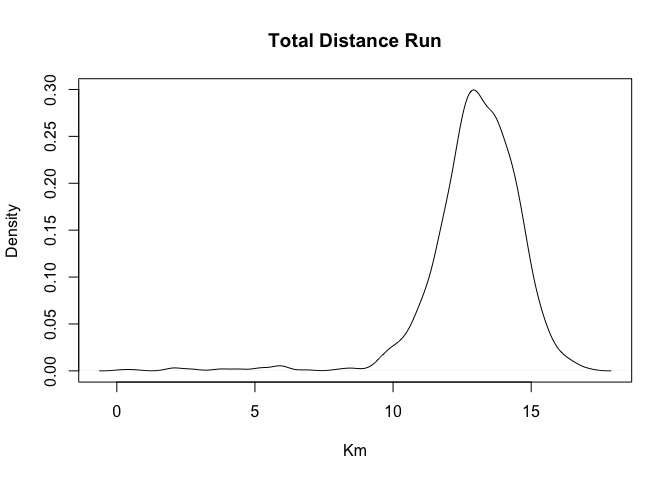
\includegraphics{Preparation_files/figure-gfm/unnamed-chunk-15-1.png}

This plot is pretty informative (we see that a player runs around 13km
in a typical game; some players run a bit more, some players run a lot
less), but it also masks a lot of cross-sectional variation. For
instance, how does the distribution of running distance vary by playing
position? With R, this sort of analysis is fairly trivial to execute -
just run a piece of code like the following:

\begin{Shaded}
\begin{Highlighting}[]
\FunctionTok{plot}\NormalTok{(}\FunctionTok{density}\NormalTok{(}\FunctionTok{filter}\NormalTok{(AFL\_data\_set, Position }\SpecialCharTok{==} \StringTok{"MIDFIELD"}\NormalTok{)}\SpecialCharTok{$}\NormalTok{GameTotalDistance\_km), }\AttributeTok{col=}\StringTok{\textquotesingle{}red\textquotesingle{}}\NormalTok{, }\AttributeTok{main=}\StringTok{\textquotesingle{}Total Distance Run\textquotesingle{}}\NormalTok{,}
     \AttributeTok{xlab=}\StringTok{\textquotesingle{}Km\textquotesingle{}}\NormalTok{)}
\FunctionTok{lines}\NormalTok{(}\FunctionTok{density}\NormalTok{(}\FunctionTok{filter}\NormalTok{(AFL\_data\_set, Position }\SpecialCharTok{==} \StringTok{"FORWARD"}\NormalTok{)}\SpecialCharTok{$}\NormalTok{GameTotalDistance\_km), }\AttributeTok{col=}\StringTok{"blue"}\NormalTok{)}
\FunctionTok{lines}\NormalTok{(}\FunctionTok{density}\NormalTok{(}\FunctionTok{filter}\NormalTok{(AFL\_data\_set, Position }\SpecialCharTok{==} \StringTok{"DEFENCE"}\NormalTok{)}\SpecialCharTok{$}\NormalTok{GameTotalDistance\_km), }\AttributeTok{col=}\StringTok{"green"}\NormalTok{)}
\FunctionTok{legend}\NormalTok{(}\StringTok{"topright"}\NormalTok{, }\AttributeTok{legend=}\FunctionTok{c}\NormalTok{(}\StringTok{"Midfield"}\NormalTok{, }\StringTok{"Forward"}\NormalTok{, }\StringTok{"Defender"}\NormalTok{),}
       \AttributeTok{col=}\FunctionTok{c}\NormalTok{(}\StringTok{"red"}\NormalTok{, }\StringTok{"blue"}\NormalTok{, }\StringTok{"green"}\NormalTok{), }\AttributeTok{lty=}\DecValTok{1}\NormalTok{, }\AttributeTok{cex=}\FloatTok{0.8}\NormalTok{)}
\end{Highlighting}
\end{Shaded}

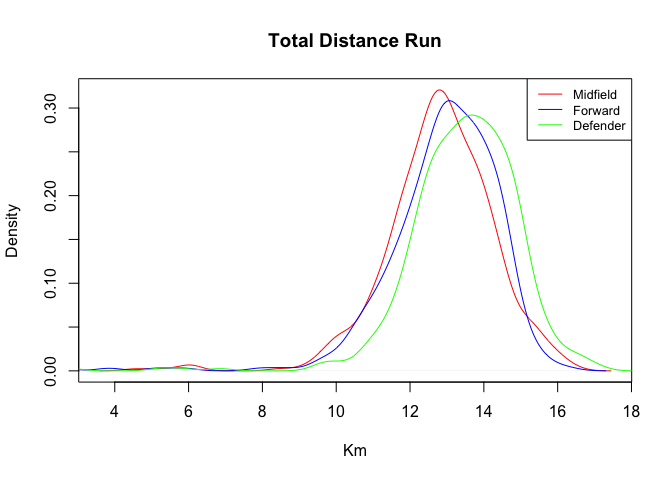
\includegraphics{Preparation_files/figure-gfm/unnamed-chunk-16-1.png}

\hypertarget{explore-relationships-between-variables}{%
\subsubsection{Explore relationships between
variables}\label{explore-relationships-between-variables}}

Most of the time when we work with data, we aren't just interested in
looking at variables by themselves. Instead, we most often want to know
how variables can be related to each other. How are variables
correlated? How can one variable be used to predict another? How does
one variable cause another? To answer these sorts of questions, we need
to understand how variables are related (we also need to impose a set of
assumptions on the underlying data generating process if we want to make
causal claims). While we won't cover the later in detail in this module
(this is a hugely important topic, but one for another class\ldots), we
will teach you how to do the former - i.e., understand whether one
variable is associated with another variable.

First, you can use plots and other visuals to understand whether
variables are associated with one another. For example, let's look at
the relationship between the total number of goals kicked by a team and
the final margin of the game. As these variables are by definition
mechanically related, we expect a strong positive relationship to show
up in our plot. To produce a scatter plot of these variables, you can
run the following code (N.B. that before you plot the raw variables, you
need to aggreate the player-level data to the team-level, hence the use
of the \texttt{group\_by()} function in the code):

\begin{Shaded}
\begin{Highlighting}[]
\NormalTok{grouped }\OtherTok{\textless{}{-}}\NormalTok{ AFL\_data\_set }\SpecialCharTok{\%\textgreater{}\%}
  \FunctionTok{group\_by}\NormalTok{(Game\_ID) }\SpecialCharTok{\%\textgreater{}\%}
  \FunctionTok{summarise}\NormalTok{(}\AttributeTok{total\_goals=}\FunctionTok{sum}\NormalTok{(Goals), }\AttributeTok{margin=}\FunctionTok{mean}\NormalTok{(Margin))}

\FunctionTok{plot}\NormalTok{(grouped}\SpecialCharTok{$}\NormalTok{total\_goals, grouped}\SpecialCharTok{$}\NormalTok{margin,}
     \AttributeTok{xlab=}\StringTok{\textquotesingle{}Total Goals\textquotesingle{}}\NormalTok{, }\AttributeTok{ylab=}\StringTok{\textquotesingle{}Margin\textquotesingle{}}\NormalTok{)}
\end{Highlighting}
\end{Shaded}

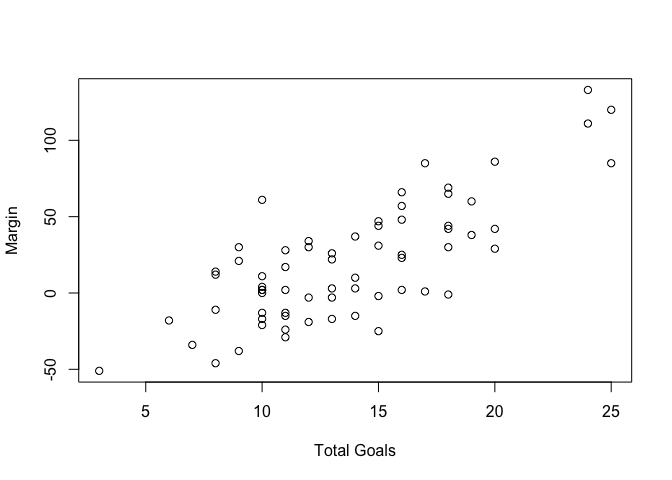
\includegraphics{Preparation_files/figure-gfm/unnamed-chunk-17-1.png}

Although it is not terribly suprising, the plot above shows a strong
positive relationship between the total number of goals a team scores
and the final margin of the game.

Second, we can quantify the association between two variables by
calculating their correlation. R provides a function that allows you to
do just this, which we use in the line of code below to look at the
association between the total number of goals a team scores and the
final margin of the game:

\begin{Shaded}
\begin{Highlighting}[]
\FunctionTok{cor}\NormalTok{(grouped}\SpecialCharTok{$}\NormalTok{total\_goals, grouped}\SpecialCharTok{$}\NormalTok{margin)}
\end{Highlighting}
\end{Shaded}

\begin{verbatim}
## [1] 0.772114
\end{verbatim}

Third, we can also use a regression to quantify the association between
two variables. A neat feature of regression is that it also allows us to
include additional variables (`controls') in the model. This can be
especially powerful if we suspect that a confounding variable is
creating (or masking) a relationship between the two variables of
interest.

In the follow examples, we will regress margin on total goals by using
the \texttt{lm()} function. The first model you will run assumes a
simple linear relationship between margin and goals; the second model
you will run allows for the weather conditions at the ground to affect
both the number of goals a team scores and the margin of the game.

\begin{Shaded}
\begin{Highlighting}[]
\FunctionTok{summary}\NormalTok{(}\FunctionTok{lm}\NormalTok{(margin}\SpecialCharTok{\textasciitilde{}}\NormalTok{total\_goals, }\AttributeTok{data =}\NormalTok{ grouped))}
\end{Highlighting}
\end{Shaded}

\begin{verbatim}
## 
## Call:
## lm(formula = margin ~ total_goals, data = grouped)
## 
## Residuals:
##     Min      1Q  Median      3Q     Max 
## -53.190 -17.445  -0.225  18.073  65.266 
## 
## Coefficients:
##             Estimate Std. Error t value Pr(>|t|)    
## (Intercept) -69.1788     9.5968  -7.208 7.42e-10 ***
## total_goals   6.4913     0.6627   9.796 2.01e-14 ***
## ---
## Signif. codes:  0 '***' 0.001 '**' 0.01 '*' 0.05 '.' 0.1 ' ' 1
## 
## Residual standard error: 24.96 on 65 degrees of freedom
## Multiple R-squared:  0.5962, Adjusted R-squared:  0.5899 
## F-statistic: 95.95 on 1 and 65 DF,  p-value: 2.012e-14
\end{verbatim}

\begin{Shaded}
\begin{Highlighting}[]
\NormalTok{grouped\_2 }\OtherTok{\textless{}{-}}\NormalTok{ AFL\_data\_set }\SpecialCharTok{\%\textgreater{}\%}
  \FunctionTok{group\_by}\NormalTok{(Game\_ID) }\SpecialCharTok{\%\textgreater{}\%}
  \FunctionTok{summarise}\NormalTok{(}\AttributeTok{total\_goals=}\FunctionTok{sum}\NormalTok{(Goals), }\AttributeTok{margin=}\FunctionTok{mean}\NormalTok{(Margin), }\AttributeTok{wind=}\FunctionTok{mean}\NormalTok{(Wind\_mph), }\AttributeTok{rainfall=}\FunctionTok{mean}\NormalTok{(Rainfall\_mm))}

\FunctionTok{summary}\NormalTok{(}\FunctionTok{lm}\NormalTok{(margin}\SpecialCharTok{\textasciitilde{}}\NormalTok{total\_goals}\SpecialCharTok{+}\NormalTok{wind}\SpecialCharTok{+}\NormalTok{rainfall, }\AttributeTok{data =}\NormalTok{ grouped\_2))}
\end{Highlighting}
\end{Shaded}

\begin{verbatim}
## 
## Call:
## lm(formula = margin ~ total_goals + wind + rainfall, data = grouped_2)
## 
## Residuals:
##     Min      1Q  Median      3Q     Max 
## -56.795 -17.069   1.109  18.009  62.065 
## 
## Coefficients:
##              Estimate Std. Error t value Pr(>|t|)    
## (Intercept) -80.26043   11.76090  -6.824 4.04e-09 ***
## total_goals   6.76716    0.68263   9.913 1.76e-14 ***
## wind          0.95891    0.60619   1.582    0.119    
## rainfall      0.04296    0.60371   0.071    0.943    
## ---
## Signif. codes:  0 '***' 0.001 '**' 0.01 '*' 0.05 '.' 0.1 ' ' 1
## 
## Residual standard error: 24.83 on 63 degrees of freedom
## Multiple R-squared:  0.6127, Adjusted R-squared:  0.5943 
## F-statistic: 33.23 on 3 and 63 DF,  p-value: 5.326e-13
\end{verbatim}

As we can see in the above output, the coefficient on total\_goals is
both positive and statistically significant at the 1\% level. This is
not a great revelation, but it nonetheless makes sense: teams that kick
more goals, win games by a greater margin.

As a quick aside, you may be wondering why the coefficient on
total\_goals is larger than six (i.e., the number of points a team
scores when they kick a goal). I'll leave it to you to work out why this
might be the case - but I will provide a hint: because game time is
finite, when a team scores a goal, this imposes an opportunity cost on
the opposition\ldots{}

\hypertarget{recap-and-conclusion}{%
\subsubsection{Recap and conclusion}\label{recap-and-conclusion}}

In this tutorial, I have shown you how to setup R, perform some basic
commands, and explore the data set we discussed in class. This should
put you in good stead to work through the exercise we are going to
tackle together next in class workshop. This exercise will deal much
more directly with many of the concepts related to performance
management that you have discussed in this course.

Hopefully, this tutorial has also given you taste for the sort of
analysis you can perform using R. As I stated earlier in class, R is a
great language that you can learn on your own using free online
resources. And, one final comment: What I have taught you has real-world
applications; in fact, it is excatly the sort of basic `data science'
work that goes on in industry. As such, many employers are very keen to
hire graduates for accounting and finance roles that have a solid grasp
of R\ldots{}

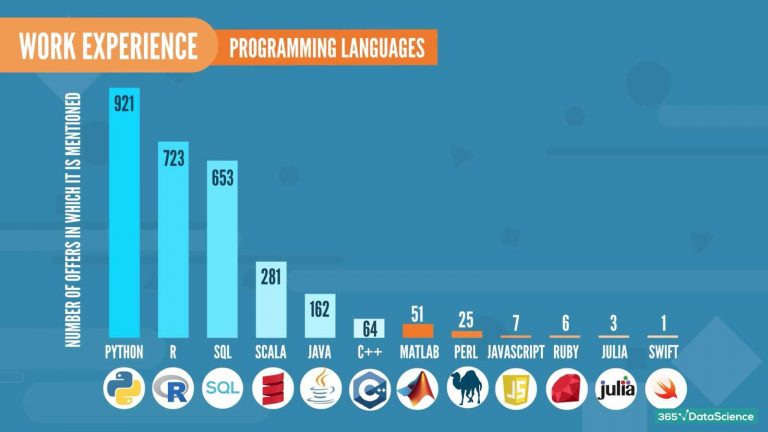
\includegraphics{Images/data_science_jobs.jpg}

\end{document}
